% Document type
\documentclass[10pt, titlepage, a4paper]{article}
	% Packages
  \usepackage{graphicx}
  \usepackage[utf8]{inputenc}
	\usepackage{amsmath}
	\usepackage{amsfonts}
	\usepackage{fancyhdr}
	\usepackage{enumerate}
	\usepackage{listings}
	\usepackage[titletoc]{appendix}
	\usepackage[margin=3cm]{geometry}
  \usepackage[absolute]{textpos}
	\usepackage[section]{placeins}
	\usepackage{url}
	\usepackage{tabularx}
%	\usepackage{gensymb}
	\usepackage{caption}
  \usepackage{subcaption}
  \usepackage{float}
  \usepackage{mathtools}

  \usepackage{algpseudocode}

  \usepackage[pdfborder={0 0 0},colorlinks=true, urlcolor=blue, citecolor=red, bookmarks=false]{hyperref}
  \hypersetup{pdftex,colorlinks=true,allcolors=blue}
  \usepackage{hypcap}

%	\usepackage{xltxtra}
	% Page style
	\pagestyle{fancy}
	\marginparsep = 0pt
  \graphicspath{ {figures/} }

	% Set font
	%\setromanfont{Calibri}

	\renewcommand\contentsname{Table of Contents}
	\newcommand{\HRule}{\rule{\linewidth}{0.5mm}}

	\newcommand{\circR}{\textsuperscript{\textregistered}}

	% Code style
	\lstset{
		backgroundcolor=\color[rgb]{0.92,0.92,0.92},
		basicstyle=\footnotesize,
		showspaces=false,
		showstringspaces=false,
		showtabs=false,
		tabsize=2,
		captionpos=b,
		breaklines=false,
		keywordstyle=\color[rgb]{0,0,1},
		commentstyle=\color[rgb]{0.133,0.545,0.133}
	}

\begin{document}
\begin{titlepage}
% Title
%\title{

\begin{center}
		\begin{figure}[t]
				
\includegraphics[width=15mm, bb=0 0 100 100]{MDHlogga.png}
		\end{figure}
                 	\Large M\"{a}lardalen University \\
			\Large School of Innovation Design and Engineering \\
                        \Large V\"{a}ster\r{a}s, Sweden\\

                        \noindent\makebox[\linewidth]{\rule{\textwidth}{0.4pt}}\\[0.5cm]

                %The complete name of the course you are enrolled in
                \Large{Bachelor Thesis}\\[2.0cm]

			\huge \textbf{\uppercase{Evolutionary computation in continuous optimization and machine learning}} \\ [2.5cm] %TITLE!!!!!!!!

			\LARGE Leslie Dahlberg \\
        	\large ldg14001@student.mdh.se \\[2.5cm]

\begin{flushleft}
			\Large Examiner: Peter Funk\\[0.5cm]
			\Large M\"{a}lardalen University\\
			\Large V\"{a}ster\r{a}s, Sweden\\[1.0cm]

			\Large Supervisor: Ning Xiong\\[0.5cm]
			\Large M\"{a}lardalen University\\
			\Large V\"{a}ster\r{a}s, Sweden\\[0.5cm]

\end{flushleft}

              \vspace*{\fill}
                    \large \today		%today should be replaced by the date the report is sent for examination

\end{center}

\end{titlepage}
%\date{}
%\maketitle

% Page style
\thispagestyle{fancy}
\fancyhead[R]{Bachelor Thesis}
\fancyhead[L]{M\"{a}lardalen University}
\fancyfoot[L]{}
%\fancyfoot[LE,RO]{\thepage}
\renewcommand{\headrulewidth}{0.4pt}
\renewcommand{\footrulewidth}{0.4pt}

% Begin actual text

\def\abstract{
   \vfil
\begin{center}%
{\bfseries\abstractname\vspace{-.5em}}
\end{center}
\itshape
}

\def\endabstract{\par
}
% ============================= Abstract ==============================
\begin{abstract}
Lorem ipsum dolor sit amet, consectetur adipiscing elit. Sed suscipit eu ante id aliquet. Class aptent taciti sociosqu ad litora torquent per conubia nostra, per inceptos himenaeos. Mauris condimentum iaculis erat, eget pretium leo consequat eget. Donec eu aliquam purus. Quisque scelerisque feugiat ligula, non vehicula urna blandit nec. Etiam a dignissim purus, at molestie dui. Vestibulum a venenatis mi, id hendrerit sem. Cras purus elit, dapibus eget est id, lacinia tincidunt neque. Mauris eu arcu ipsum. Sed enim leo, iaculis vitae nisl tincidunt, ultricies accumsan diam. Donec neque urna, pellentesque sit amet interdum a, pretium ac enim. Proin quis ante nunc. Fusce vitae lorem condimentum, porta velit blandit, commodo nisi.
\end{abstract}
\newpage
% ========================== Document version ===========================
%\begin{center}
%	\begin{tabular}{|l|l|l|}
 %
	%	\multicolumn{3}{c}{\textbf{{\large Document version}}} \\
	%	\hline
 	%	Version & Date & Note \\ \hline
 	%	 &  &  \\ \hline
	%	 &  &  \\ \hline
	%	 &  &  \\ \hline
	%	 &  &   \\ \hline
	%	 &  &   \\ \hline
	%	 &  &   \\ \hline
%	\end{tabular}
%\end{center}
%\newpage
%========================== Table of contents ===========================
\hypersetup{linkcolor=black}
\tableofcontents
\hypersetup{linkcolor=red}

\newpage

% ============================== Intro ===============================

\section{Introduction}

Optimization is a problem-solving method which aims to find the most advantageous parameters for a given model. The model is known to the optimizer and accepts inputs while producing outputs. Usually the problem can be formulated in such a way that we seek to minimize the output value of the model or the output of some function which transforms the models output into a fitness score. Because of this the process is often referred to as minimization. It becomes obvious that this is useful when considering optimizing the layout of a circuit in order to minimize the power consumption. To achieve this the optimizer looks for combinations of parameters which let the model produce the best output to a given input~\cite{Eiben2015_origins}.


When dealing with simple mathematical models, optimization can be achieved using analytical methods, often calculating the derivative of the functional model, but these methods prove difficult to adapt to complex models which exhibit noisy behavior. Additionally, the analytical model is not always known, which makes it impossible to use such methods~\cite{xiong2015walk}. The field of evolutionary computation (EC), a subset of computational intelligence (CI), which is further a subset of artificial intelligence (AI), contains algorithms which are well suited to solving these kinds of optimization problems~\cite{Michalewicz1997,zhang2015comprehensive}.

Evolutionary computation focuses on problem solving algorithms which draw inspiration from natural processes. It is closely related to the neighboring field of swarm intelligence (SI), which often is, and in this thesis will be, included as a subset of EC. The basic rationale of the field is to adapt the mathematical models of biological Darwinian evolution to optimization problems. The usefulness of this can be illustrated by imagining that an organism acts as an ``input'' to the ``model'' of it's natural environment and produces an ``output'' in the form of offspring. Through multiple iterations biological evolution culls the population of organisms, only keeping the fit specimen, to produce organisms which become continuously better adapted to their environments. Evolutionary computation is, however, not merely confined to Darwinian evolution, but also includes a multitude of methods which draw from other natural processes such as cultural evolution and animal behavior~\cite{engelbrecht2007computational}.

The purpose of this thesis is to explore the performance and usefulness of three emerging evolutionary algorithms: differential evolution, particle swarm optimization and estimation of distribution algorithms. These algorithms are newer inventions inspired by genetic algorithms, evolution strategy, evolutionary programming and genetic programming. Differential evolution is a straight-forward evolutionary algorithm which uses simple mathematic vector calculations to achieve it's results, while particle swarm optimization tries to mirror the behavior of swarming animals and estimation of distribution uses probability distributions to guess it's way forward. The intention is to test and compare these against each other on a set of standard mathematical benchmark functions and practical problems in machine learning involving neural networks and game controllers and then, if possible, develop a new or modified algorithm which improves upon the aforementioned ones in some aspect.

Research has been conducted on improving various evolutionary algorithms by hybridizing and extending them, which has resulted in a wide array of algorithms for both specific and general purposes. Since these algorithms accepts parameters which modify their efficiency, studies have been carried out which compare different combinations of parameters. My thesis will draw upon this work by comparing three algorithms both generally and on a very specific problem.

The results from the benchmark show which algorithm is best suited to handle various machine learning problems and presents the advantages of using the new algorithm. The new algorithm called DEDA (Differential Estimation of Distribution Algorithms) has shown promising results at both machine learning and mathematical optimization tasks.

\newpage
\section{Background}

This section will aim to provide a general overview of the field of evolutionary compution. General terms and procedured which are often utizilied in EC will be explained and the most well known traditional approaches will be presented. Current research will also be introduced. The emerging algorithms relevant to this thesis can be found in the section ``Algorithms''.

\subsection{Evolutionary Algorithms}

Evolutionary algorithms work on the concept of populations. A population is a set of individuals which in the case of optimization problems contain a vector of parameters which the model we wish to optimize can accept and transform into an output. The population is initialized by some procedure to contain a random set of parameter vectors, these should cover the whole parameter range of the model uniformely. The inital population is evaluated and an iterative process is started which continues as long as no suitable solution is found. During this iterative process the current population is selected, altered and evaluated. During selection a set of individuals which display promising characterisitcs are selected to live on to the next generation of the population. They are then altered randomly to create diversity in the population and evaluated. This process creates a new generation of the population on each iteration and continues until a solution is found or some other restriction is encoutered~\cite{Eiben20021}. The concept is demonstrated in figure~\ref{algo:basicevolution} with $P(t)$ representing the population at generation $t$.

\begin{algorithm}[h]

  \caption{Basic evolutionary algorithm}
  \label{algo:basicevolution}
    \begin{algorithmic}
       \State $t\gets 0$
       \State initialize $P(t)$
       \State evaluate $P(t)$
       \While{termination-condition not fulfilled}
        \State $t\gets t + 1$
        \State select $P(t)$ from $P(t-1)$
        \State alter $P(t)$
        \State evaluate $P(t)$
       \EndWhile
    \end{algorithmic}

\end{algorithm}

Here the fundamental builing blocks of evolutionary algorithms will be presented and explained. Most of these term are universal to all approaches which will be covered in this thesis and neccesary to properly understand them.

\subsubsection{Representation}

The first step in using evolutionary algorithms is creating a representation which can encode all possible solutions to the problem at hand. Here two different terms are distinguished. The term phenotype denotes the representation that can be directly applied to the problem and the genotype denotes the specific encoding of the phenotype which is manipulated inside the evolutionary algorithm. In optimization tasks a valid phenotype could be a vector of integer numbers which act as parameters to a function while the genotype would be a binary representation of the numbers which can be altered by manipulating individuals bits. The terms phenotype, candidate solution and individual are used interchangably to denote the representation as used by the model while chromosome, genotype and individual are used to refer to the representation inside the evolutionary algorithm~\cite{Eiben2015_whatevolutionary}.

\paragraph{Binary representation}

Genetic algorithms (GA) traditionally use a binary representation to store individual genotypes. The representations is a string of fixed length over the alphabet $\{0,1\}$. The problem thus becomes a boolean optimziation problem of the form $ f:\{0,1\}^l \rightarrow \mathbb{R}$, where the mappings $h:M \rightarrow \{0,1\}^l$ and $h':\{0,1\}^l \rightarrow M$ are used to encode and decode the parameters and solutions~\cite{back1997evolutionary}.

\paragraph{Integer representation}

Integer representations have been proposed by some researches~\cite{unter611evolutionary}. This approach is usefull when dealing with problems where we need to select certain elements in a particular order, e.g. graph-problems, path-finding problems, the knapsack problem, etc.~\cite{Eiben201511}.


\paragraph{Real-valued representation}

Real-valued or floating-point representations were originally used in evolutionary programming and evolution strategies and work well for problems located in continuous search-spaces. The problems take the form $f:M\subseteq \mathbb{R}^n \rightarrow \mathbb{R} $~\cite{back1997evolutionary}.

\paragraph{Tree representation}

Tree representations are mainly used in genetic programming to capture the structure of programs. The econding varies but S-expressions are generally used. The tree structure is defined by a function-set and a terminal-set. The function-set defines the types of nodes in the tree, while the terminal-set contains the types of leaves the tree can contain~\cite{Eiben201511}.

\subsubsection{Evaluation function}

The evalutation function is responsible for improvement in the population. It is a function which assigns a fitness or cost value to every genotype and thus enables us to compare the quality of the genotypes in the population. It is also the only information about the problem that is available to the evolutionary algorithm and should therefore include all domain knowledge which is available about the problem~\cite{Eiben2015_whatevolutionary}. The evaluation is also the process which takes up the most computational resources, 99\% of the total computational cost in real-world problems~\cite{Eiben20021}.

\subsubsection{Population}

The population is a set of genotypes which contain the current best solutions to a problem. While genotypes remain stable and unchanging, the population continually changes through the application of selection mechanisms which decide which genotypes are allowed into the next generation of the population. The size of the population almost always remains constant during the lifetime of the algorithm. This in turn creates selection pressure which pushes the population to improve. A population's diversity is the measure of difference amoung the genotypes, phenotypes and fitness values~\cite{Eiben2015_whatevolutionary}.

\paragraph{Steady-state model}

In the steady-state model the entire population isn't replaces at once, rather only a fraction of the population is replaces a one time.

\paragraph{Generational model}

In the generational model the entire population is replaces at once.

\subsubsection{Parent selection mechanism}

Parent selection serves to improve the quality of a population by selecting which individuals will survive into the next generation. The selected individuals are called parents as they usually undergo some form of alteration or combination with other individuals before progressing to the next generation. The selection method is usually probabilistic and gives better solutions a higher probability and worse solutions a lower probability to survive. It's important that bad solutions still recieve a positive probabilty since the population might otherwise lose diversity and coalesce around a false local optimimum~\cite{Eiben2015_whatevolutionary}.


\subsubsection{Variation operators}

Variation operators introduce new features into the genotypes of a population by modifying or mixing existing genotypes. They can be divided into two types: unary operators which take one genotype and stochastically alter it to introduce random change and n-ary operators which mix the features of 2 or more genotypes. Unary operators are called mutation operators while n-ary operators are called cross-over or recombination operators. The biological equivalents to these are random mutation and sexual reproduction. Mutation operators allow evolutionary algorithms to theoretically span the whole continuum of the search space by giving a non-zero probability that a genotype mutates into any other other genotype. This has been used to formally prove that evolutionary algorithms will always reach the desired optimum given enough time. Recombination tries to create new superior individuals by combining the genes of two good parent genotypes~\cite{Eiben2015_whatevolutionary, Eiben20021}.

\subsubsection{Survivor selection mechanism}

Survivor selection takes place after new offspring have been generated and determines which individuals are allowed to live on into the next generation. It is often refered to as the replacement strategy and contrary to parent selection it is usually deterministic. Two popular mechanisms are fitness-based selection and age-based selection. Fitness-based selection determines the next generation by selecting the individuals with the highest fitness while age-based selection allows only the offspring to survive~\cite{Eiben2015_whatevolutionary}.



\subsubsection{Initatilization}

Initialization is the process during which the intial population is generated. The genotypes are usually generated randomly from a uniform distribution based on some range of acceptable input values. If a good solution is known before hand variations of it can be include in the initial population as a bias, but this can sometimes cause more problems than it solves~\cite{Eiben20021}.

\subsubsection{Termination condition}

The termination condidion determines for how long the algorithm is run. Four criteria are used to determine when to stop~\cite{Eiben2015_whatevolutionary}:

\begin{enumerate}
  \item If a maximum number CPU-cycles or iterations is reached
  \item If a known optimum is reached
  \item If the fitness value does not improve for a considerable amount of time
  \item If the diversity of the polation drops below a given threshold
\end{enumerate}

\subsection{Traditional Evolutionary Algorithms}

Below the main paradighms of evolutionary computation will be discussed. They include genetic algorithms, evolution strategy, evolutionary programming and genetic programming.

\subsubsection{Genetic algorithms}

Genetic algorithms (GA) were introduced by John Holland in the 1960s as an attempt to apply biological adaptation to computational problems. GAs are multidemensional search algorithms which use populations of binary strings called chromosomes to evolve a solution to a problem. GAs use a selection operator, a mutation operator and a cross-over operator. The selection operator select individuals which are subjected to cross-over based on their fitness and cross-over combines their genetic material to form new individuals which are then randomly mutated~\cite{mitchel1999evolutionary}. See algorithm~\ref{algo:geneticalgorithm} and figure~\ref{fig:GA} for a simple GA.

\begin{figure}[H]
  \centering
  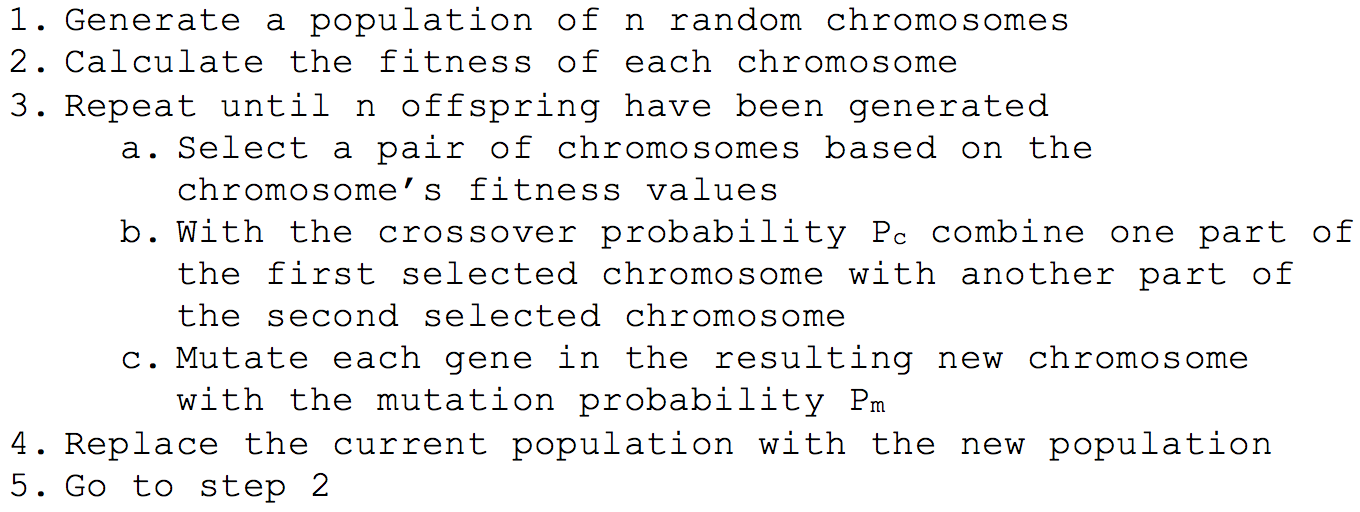
\includegraphics[width=.5\linewidth]{GA}
  \caption{Stages in GA (1) Evalution (2) Selection (3) Crossover (4) Mutation}
  \label{fig:GA}
\end{figure}

\begin{algorithm}[h]

  \caption{Basic genetic algorithm}
  \label{algo:geneticalgorithm}
    \begin{algorithmic}
       \State Initialize a population of N binary chromosome with L bits
       \While{termination-condition not fulfilled}
        \State Evaluate the fitness $F(x)$ of each chromosome $x$
        \Repeat
          \State Select two chromosomes probabilistally from the population
          \State based on their fitness
          \State With the cross-over probability $P_c$ create two new offspring
          \State from the two selected chromosomes using the crossover operator.
          \State Otherwise create two new offspring identical to their parent chromosomes.
          \State Mutate the two chromosomes using the mutation probability $P_m$
          \State and place the resulting chromosomes into the new population
        \Until{N offspring have been created}
        \State Replace the old population with the new population
       \EndWhile
    \end{algorithmic}
\end{algorithm}

\subsubsection{Evolution strategy}

Evolution strategies (ES) were first developed to solve parameter optimization tasks. They differ from GAs by representing individuals using a pair of vectors $\vec{v} = (\vec{x},\vec{\sigma})$. The earliest versions of ES used a population of only one individual and only utilized the mutation operator. New individuals were only introduced into the population if they performed better than their parents. The vector $\vec{x}$ represents the position in the search space and $\vec{\sigma}$ represents a vector of standard deviations used to generate new individuals. Mutation occurs according to equation~\ref{eq:evolutionstrategy1} where $N(0,\vec{\sigma})$ is a vector containing random Gaussian numbers with the mean $0$ and a standard deviation of $\vec{\sigma}$~\cite{Michalewicz1997}.

\begin{equation}
  \vec{x}^{t+1} =  \vec{x}^{t} + N(0,\vec{\sigma})
  \label{eq:evolutionstrategy1}
\end{equation}

Newer versions of the algorithm include $(\mu + \lambda)-\text{ES}$ and $(\mu,\lambda)-\text{ES}$. The main point of these it that their parameters like mutation variance adapt automatically to the problem. In $(\mu + \lambda)-\text{ES}$ $\mu$ parents generate $\lambda$ offspring and the new generation is selected from $\mu$ and $\lambda$ while in $(\mu,\lambda)-\text{ES}$ $\mu$ parents generate $\lambda$ offspring ($\lambda > \mu$) and the new generation is only selected from $\lambda$. These algorithms produce offspring by first applying cross-over to combine two parent chromosomes (including their deviation vectors $\vec{\sigma}$) and then mutating $\vec{x}$ and $\vec{\sigma}$~\cite{Michalewicz1997}.

\subsubsection{Evolutionary programming}

Evolutionary programming (EP) was created as an alternative approach to artificial intelligence. The idea was to evolve finite state machines (FSM) which observe the environment and elicit appropriate responses~\cite{Fogel1996}. The environmet is modeled as a sequence of input characters selected from an alphabet and the role of the FSM is to produce the next character in sequence. The fitness of an FSM is measured by a function which tests the FSM on a sequence of input characters, starting with the first character and then progressing to include one more addition character on each iteration. The function measures the correct prediction rate of the FSM and determines it's score~\cite{Michalewicz1997}.

Each FSM creates one offspring which is mutated by one or more of the following operators: change of input symbol, change of state transition, addition of state, deletion of state and change of initial state. The next generation is then selected from the pool of parents and offspring, selecting the best 50\% of all available solutions. A general form of EP has recently been devised which can tackle continuous optimization tasks~\cite{Michalewicz1997}.

\subsubsection{Genetic programming}

Genetic programming (GP) differs from traditional genetic algorithms by evolving computer programs which solve problems instead of directly finding the solution to a problem. The individuals in the population are therefore data-structures which encode computer programs, usually rooted trees representing expressions~\cite{Michalewicz1997}.

At it's most basic the programs are defines as functions which take a set of input parameters and produce an output. The programs are constructed from building blocks such as variables, numbers and operators. The initial population contains a set of such programs which have been initialized as random trees~\cite{Michalewicz1997}.

\begin{figure}[H]
  \centering
  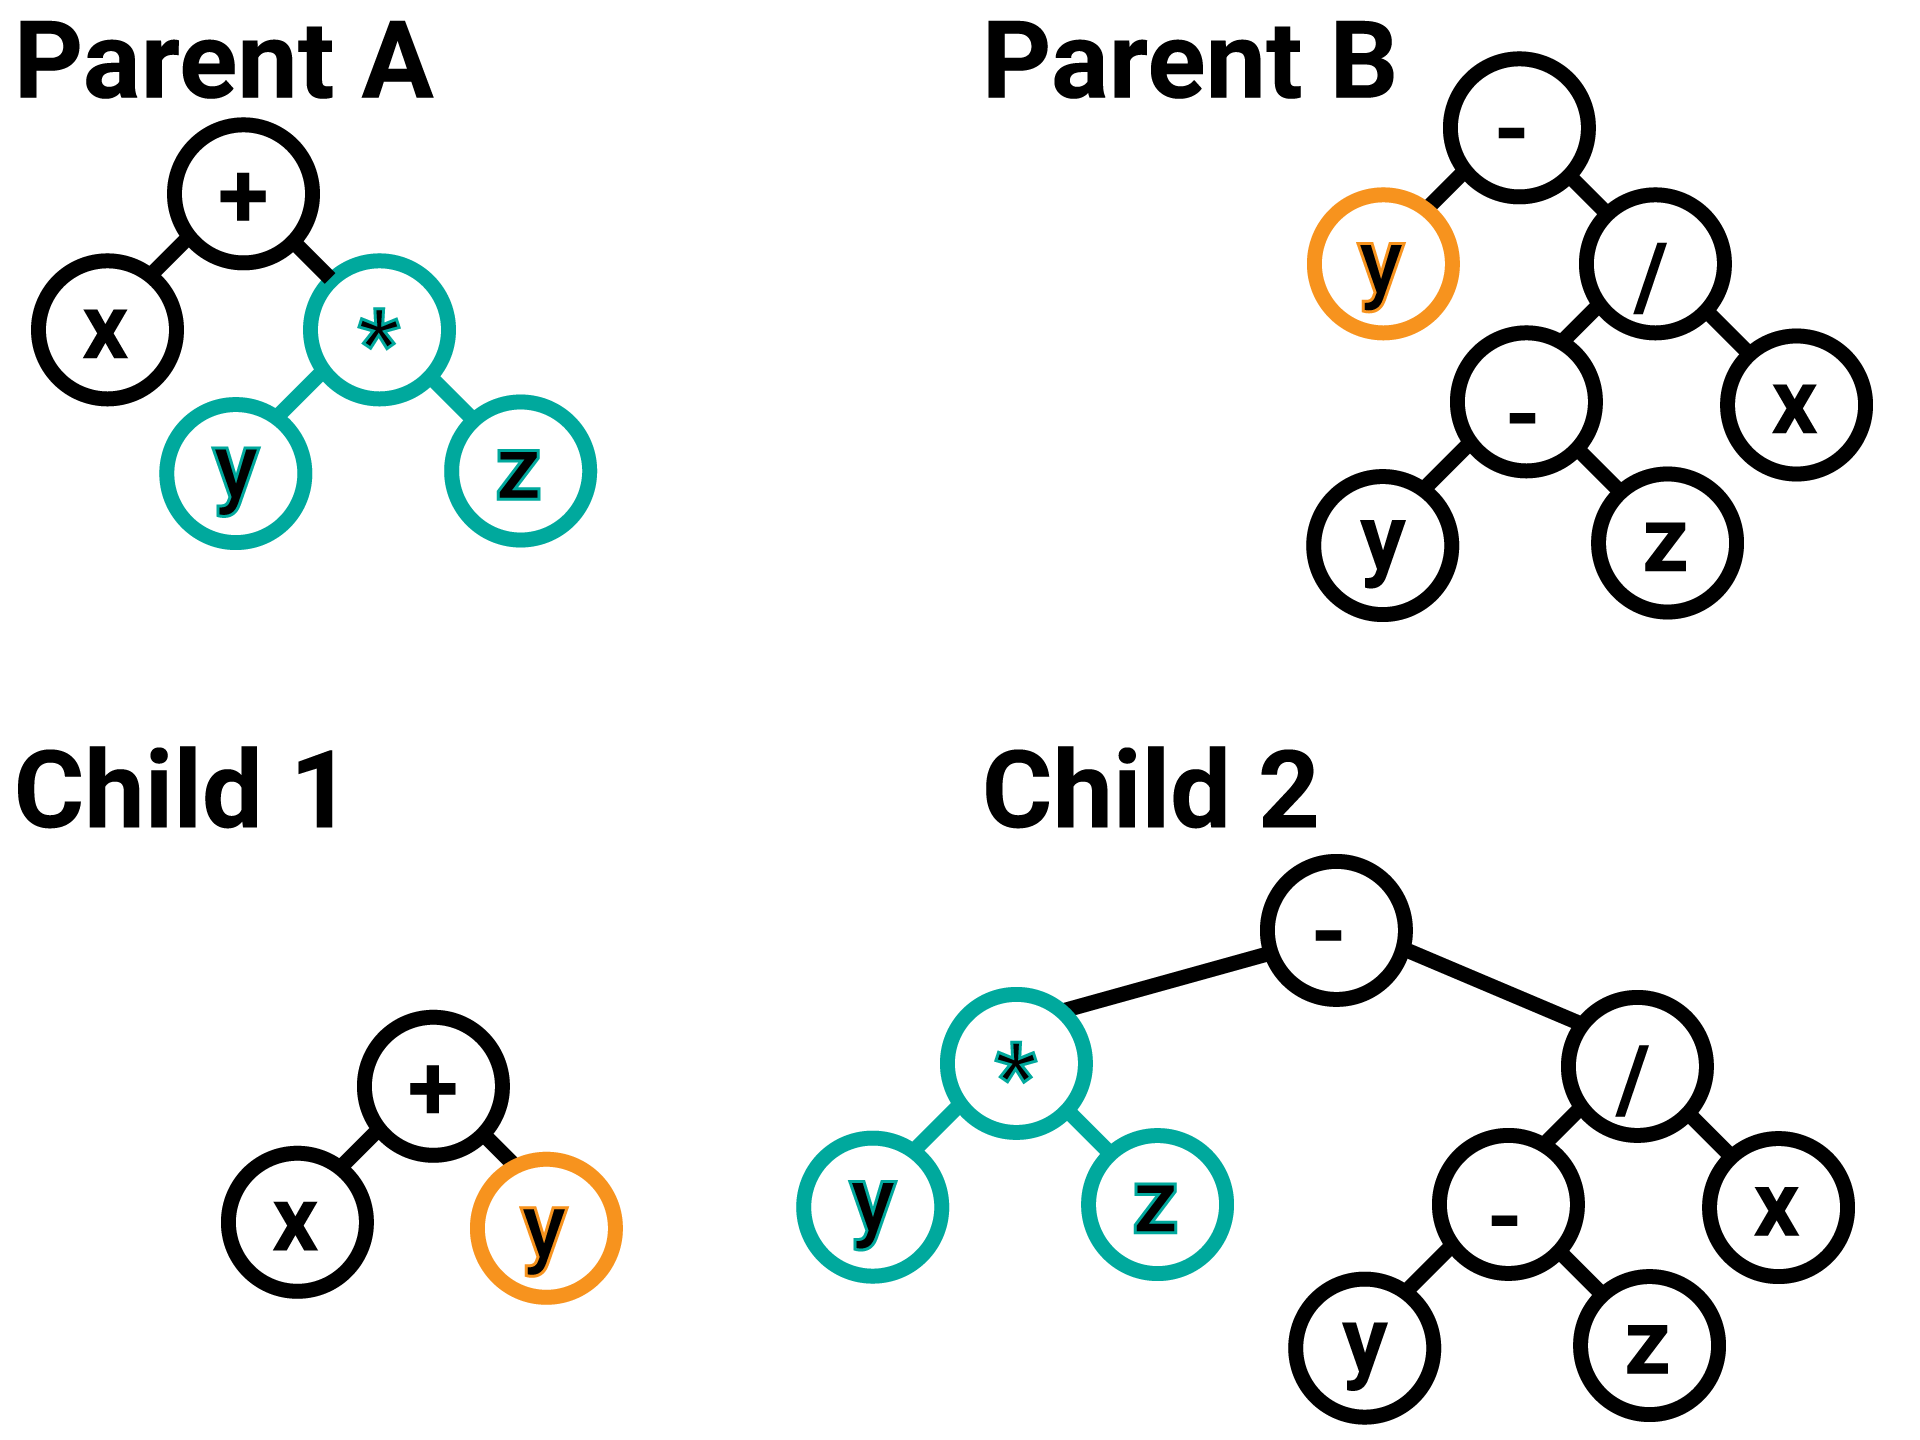
\includegraphics[width=.5\linewidth]{GP}
  \caption{Crossover in GP with two parents producing two offspring}
  \label{fig:GP}
\end{figure}

The evolution process is similar to GAs in that the programs are evaluated using a function which runs a set of test cases and the programs undergo cross-over and other mutations. Cross-over is defined as the exchange of subtrees between programs and produces two offspring from two parents~\cite{Michalewicz1997}, see figure~\ref{fig:GP}.

More advanced versions of GP include function calls which enable the programs to remember useful symmetries and regularities and facilitate code reuse~\cite{Michalewicz1997}.

\subsection{Emerging Evolutionary Algorithms}

This section describes the three algorithms which were benchmarked together with my own algorithm contribution. The Matlab code can be viewed in appendix \ref{appendix:algorithms}.

\subsubsection{Differential Evolution}

Differential evolution~\cite{Storn1997} is a stochastic optimization algorithm which works on populations of parameter vectors. The problem to minimize will be denoted by $f(x)$ where $X=[x_1,x_2,x_3,...x_D]$ and $D$ is equal to the number of variables taken as input parameters by $f(x)$. The algorithm consists of multiple steps which will be described in detail below.

The first step in DE is to create an initial population, the size of the population is $N$ and it will be represented by a matrix $x$ where $g$ is the generation and $n=1,2,3,...,N$:

\begin{equation}
x_{n,i}^{g} = [ x_{n,1}^{g}, x_{n,2}^{g}, x_{n,3}^{g}, ..., x_{n,D}^{g} ]
\end{equation}

The population is randomly generated to uniformly fill the entire parameter space ($x_{n,i}^U$ is the upper bound for parameter $x_i$ and $x_{n,i}^L$ is the lower bound for parameter $x_i$):

Mutation is the first step when creating a new generation from the population. Mutation is performed individually for every vector $x$ in the population. The mutation procedure is as follows: select three random vectors for each parameter vector (this requires that the population has a size of $N > 3$) and create a set of new vectors $v$ called mutant vectors according to the formula below where $n=1,2,3,...,N$:

\begin{equation}
v_{n}^{g+1} = [ x_{r1n}^{g} + F(x_{r2n}^{g} - x_{r3n}^{g})
\end{equation}

The value of $F$ can be chosen from the interval $[0,2]$ and determines the influence of the differential weight $(x_{r2n}^{g} - x_{r3n}^{g})$.

Crossover occurs after mutation and is applied individually to every vector $x$. A new vector $u$ called the trial vector is constructed from the mutant vector $v$ and the original vector $x$. The trial vector is produced according to the formula below with $i=1,2,3,...,D$ and $n=1,2,3,...,N$:

\begin{equation}
    u_{n,i}^{g+1} =
    \begin{cases}
      v_{n,i}^{g+1}, & \text{if}\ rand() \leq CR \wedge i = I_{\text{rand}} \\
      x_{n,i}^{g}, & \text{otherwise}
\end{cases}
\end{equation}

$I_{\text{rand}}$ is a randomly selected index from the interval $[1,D]$ and $CR$ is the crossover constant which determines the probability that an element is selected from the mutant vector.

Selection is the last step in creating a new generation. The trial vector $u$ is compared with the original vector $x$ for fitness and the vector with the lost cost is selected for the generation according to the formula below where $n=1,2,3,...,N$:

\begin{equation}
    x_{n}^{g+1} =
    \begin{cases}
      u_{n}^{g+1}, & \text{if} f(u_{n}^{g+1}) < f(x_{n}^{g}) \\
      x_{n,i}^{g}, & \text{otherwise}
\end{cases}
\end{equation}

After selection is performed for every vector in the population the population is evaluated to determine if an acceptable solution has been generated. If a solution has been found the algorithm terminates, otherwise the mutation, crossover and selection is performed again until a solution is found or a maximum number of iterations has been reached.

In the benchmark the parameters for DE have been set to $F = 0.6$ and $CR=0.9$ as recommended by Gamperle et al.~\cite{gamperle2002parameter}.

\paragraph{Variants}

Different DE schemes are classified as DE/x/y, where x symbolizes the vector which is mutated and y is the number of differential vectors used. The value of x can be ``rand'' for random vector or ``best''' for the best vector in the population. The algorithm abose is therefore classified as DE/rand/1. The variant DE/best/2 is considered to be a good alternative to DE/rand/1~\cite{qin2009differential}. It's mutation equation is described below:

\begin{equation}
v_{n}^{g+1} = [ x_{best}^{g} + F(x_{r1n}^{g} - x_{r2n}^{g}) + F(x_{r3n}^{g} - x_{r4n}^{g})
\end{equation}

\subsubsection{Particle Swarm Optimization}

Particle Swarm Optimization (PSO)~\cite{Das2008} was introduced in 1995 by Kenneth and Ebenhart~\cite{eberhart1995new}. The optimization problem is represented by an n-dimensional function

\begin{equation}
  f(x_1,x_2,x_3,...x_n) = f(\vec{X})
\end{equation}

where $\vec{X}$ is a vector which represents the real parameters given to the function. The intent is to find a point in the n-dimensional parameter hyperspace that minimizes the function.

PSO is a parallel search technique where a set of particles  fly through the n-dimensional search space and probe solutions along the way. Each particle $P$ has a current position $\vec{x}(t)$, a current velocity $\vec{v}(t)$, a personal best position $\vec{p}(t)$ and the neighborhoods best position $\vec{g}(t)$. A neighborhood $N$ is a collection of particles which act as independent swarms. Neigborhoods can be social or geographical. Social neigborhoods do not change and contain the same particles during the entire optimization process, while geographical neighborhoods are dynamic and consist only of particles which are near to one another. The neighborhood is often set to be identical to the whole swarm of particles, denoted $S$.

\begin{figure}[H]
  \centering
  \includegraphics[width=.3\linewidth]{pso}
  \caption{Illustration of particles in PSO (red represents the best particle)}
  \label{fig:pso}
\end{figure}

The algorithm has a set of general properties: $v_{max}$ restricts the velocity of each particle to the interval $[-v_{max},v_{max}]$, an inertial factor $\omega$, two random numbers $\phi_1$ and $\phi_2$ which affect the velocity update formula by modulating the influence of $\vec{p}(t)$ and $\vec{g}(t)$, and two constants $C^2$ and $C^1$ which are termed particle “self-confidence” and “swarm confidence”.

The initial values of $\vec{p}(t)$ and $\vec{g}(t)$ are equal to $\vec{x}(0)$ for each particle. After the particle have been initialized an iterative update process is started which modifies the positions and velocities of the particles. The formula below describes the process ($d$ is the dimension of the position and velocity and $i$ is the index of the particle):

\begin{equation}
  v_{id} (t+1) = \omega v_{id} (t) + C_1 \phi_1 (p_{id} (t) - x_{id} (t)) + C_2 \phi_2 (g_{id} (t) - x_{id} (t))
\end{equation}

\begin{equation}
  x_{id} (t+1) = x_{id} (t) + v_{id} (t+1)
\end{equation}

The “self-confidence” constant affects how much self-exploration a particle is allowed to do while “swarm-confidence” affects how much a particle follows the swarm. $\phi_1$ and $\phi_2$ are random numbers which push the particle in a new direction while $\omega$ keeps a particle on the path it’s currently on. The PSO algorithm is described in algorithm~\ref{algo:pso}. See figure~\ref{fig:pso} for an illustration of PSO.

\begin{algorithm}[h]
  \caption{PSO algorithm}
  \label{algo:pso}
    \begin{algorithmic}
      \State Init particals with random postitions
      $\vec{x}(0)$ and velocities $\vec{v}(0)$
      \Repeat
        \ForAll{Particles $i$}
          \State Evaluate fitness $f(\vec{x_i})$
          \State Update $\vec{p}(t)$ and $\vec{g}(t)$
          \State Adapt the velocity of the particle using the above-mentioned equation
          \State Update the position of the particle
        \EndFor
      \Until{$\vec{g}(t)$ is a suitable solution}
    \end{algorithmic}
\end{algorithm}



In the benchmark the parameters for PSO have been set to $\omega = 0.8$~\cite{shi1998modified}, $c_1 = c_2 = 1.494$~\cite{kennedy1999small} and $v_{max} = \text{parameter range size}$~\cite{Das2008}.

\subsubsection{Estimation of Distribution Algorithm}

Estimation of distribution algorithms are stochastic search algorithms which try to find the optimal value of a function by creating and sampling probability distributions repeatedly. The first step is creating population $P(0)$ and filling it with solution parameter vectors created from a probability distribution which covers the whole search space uniformly. Then all solutions in $P(g)$ are evaluated and the best solutions $S(g)$ are selected (a threshold variable $t$ is used to determine how many solutions are selected, setting $t=50\%$ means that the best 50\% of the solutions are selected). After selection a probabilistic model $M(g)$ is constructed from $S(g)$ and new solutions $O(g)$ are sampled from $M(g)$. Finally $O(g)$ is incorporated into $P(g)$ The generation counter is incremented $g = g + 1$ and the selection, model and sampling stages are repeated until a suitable solution is found~\cite{Hauschild2011111}.

The most difficult part is constructing the probabilistic model, this will differ for continuous and discreet optimization and a model of appropriate complexity has to be chosen depending on the nature of the problem. The simplest method for continuous EDAs is using a continuous Univariate Marginal Density Algorithm (UMDA). However depending on the complexity of the problem other methods such as Estimation of Baysian Networks (EBNA) can be used~\cite{larranaga2012review}.

\paragraph{UMDA}
The UMDA algorithm is an EDA algorithm which uses a set of independent probability distributions to sample new solution vectors. The probability model can be expressed as a product of the individual probabilities

\begin{equation}
  p(x) = \prod _{d=1}^D {p_d(x_d)}
\end{equation}

where $p(x)$ is the global multivariate density, D is the vector length and $p_d(x_d)$ are the individual univariate marginal densities~\cite{povsik2004estimation}. The algorithm is described in algorithm~\ref{algo:umda}.

\begin{algorithm}[h]
  \caption{UMDA algorithm}
  \label{algo:umda}

    \begin{algorithmic}
      \State Initialize population P
      \Repeat
        \State Evaluate P
        \State Select the best t\% of P into S
        \State Let m be the mean S
        \State Let s be the standard deviation of S
        \State Sample S' from normal distribution using m and s
        \State Create new generation of P from S' and S
      \Until{Termination condition}
    \end{algorithmic}

\end{algorithm}

\subsection{Method}

A benchmark was constructed to perform the algorithm comparison. Both mathematical function optimization and machine learning test-sets were used. These are described in detail in the section \ref{section:benchmark}. Matlab was used to implement the algorithms and benchmarks because it provides easy access to important mathematical and scientific constructs which are usually not available in conventional programming languages. Matlab is also widely used in the field of evolutinary computation.
 %SOTA
\newpage
\section{Method}

A benchmark was constructed to compare the algorithms. Two distict problem sets were used: 1. Mathematical functions and 2. Machine learning problems. The algorithms, the problem sets and the benchmark program were developed in Matlab. Matlab was chosen because it works well for scientific computation and provides convenient access to features which are needed to solve the problems at hand (manipulating matrices, measuring performance, parallel computing, dynamic data-structures, probability distributions, etc.).

To ensure that the results are accurate and usefull the benchmark was run in the following way:

\begin{itemize}
  \item Benchmark at dimension 10, 30 and 50
  \item Benchmark at population size $100 + dimension * 5$
  \item Set maximum number of generations to $10000 * dimension / population size$ to ensure the number of evaluations remains constant throughout the benchmark
  \item Run each algorithm 30 times on each problem and record averages and standard deviations
\end{itemize}

\newpage
% =========================== Actual Content ==========================

\section{Theory}

This section describes the three algorithms which were benchmarked together with my own algortihm contribution.

\subsection{Differential Evolution}

Differential evolution is a stochastic optimization algorithm which works on populations of parameter vectors. The problem to minimize will be denoted by $f(x)$ where $X=[x_1,x_2,x_3,...x_D]$ and $D$ is equal to the number of variables taken as input parameters by $f(x)$. The algorithm consists of multiple steps which will be described in detail below, the flow of the algorithm is illustrated in figure \ref{figure:DE}.

\begin{figure}[h]
  \centering
  \begin{minipage}{5cm}
    \begin{algorithmic}
      \State Initialize population
      \Repeat
        \State Cross-over
        \State Selection
        \State Create new generation
      \Until{Solution is found}
    \end{algorithmic}
  \end{minipage}
  \caption{Overview of differential evolution algorithm.}
  \label{figure:DE}
\end{figure}

The first step in DE is to create an initial population, the size of the population is $N$ and it will be represented by a matrix $x$ where $g$ is the generation and $n=1,2,3,...,N$:

\begin{equation}
x_{n,i}^{g} = [ x_{n,1}^{g}, x_{n,2}^{g}, x_{n,3}^{g}, ..., x_{n,D}^{g} ]
\end{equation}

The population is randomly generated to uniformly fill the entire parameter space ($x_{n,i}^U$ is the upper bound for parameter $x_i$ and $x_{n,i}^L$ is the lower bound for parameter $x_i$):

Mutation is the first step when creating a new generation from the population. Mutation is performed individually for every vector $x$ in the population. The mutation procedure is as follows: select three random vectors for each parameter vector (this requires that the population has a size of $N > 3$) and create a set of new vectors $v$ called mutant vectors according to the formula below where $n=1,2,3,...,N$:

\begin{equation}
v_{n}^{g+1} = [ x_{r1n}^{g} + F(x_{r2n}^{g} - x_{r3n}^{g})
\end{equation}

The value of $F$ can be chosen from the interval $[0,2]$ and determines the influence of the differential weight $(x_{r2n}^{g} - x_{r3n}^{g})$.

Crossover occurs after mutation and is applied individually to every vector $x$. A new vector $u$ called the trial vector is constructed from the mutant vector $v$ and the original vector $x$. The trial vector is produces according to the formula below with $i=1,2,3,...,D$ and $n=1,2,3,...,N$:

\begin{equation}
    u_{n,i}^{g+1} =
    \begin{cases}
      v_{n,i}^{g+1}, & \text{if}\ rand() \leq CR \wedge i = I_{\text{rand}} \\
      x_{n,i}^{g}, & \text{otherwise}
\end{cases}
\end{equation}

$I_{\text{rand}}$ is a randomly selected index from the interval $[1,D]$ and $CR$ is the crossover constant which determines the probability that an element is selected from the mutant vector.

Selection is the last step in creating a new generation. The trial vector $u$ is compared with the original vector $x$ for fitness and the vector with the lost cost is selected for the generation according to the formula below where $n=1,2,3,...,N$:

\begin{equation}
    x_{n}^{g+1} =
    \begin{cases}
      u_{n}^{g+1}, & \text{if} f(u_{n}^{g+1}) < f(x_{n}^{g}) \\
      x_{n,i}^{g}, & \text{otherwise}
\end{cases}
\end{equation}

After selection is performed for every vector in the population the population is evaluated to determine if an acceptable solution has been generated. If a solution has been found the algorithm terminates, otherwise the mutation, crossover and selection is performed again until a solution is found or a maximum number of iterations has been reached \cite{Storn1997}.

\subsection{Particle Swarm Optimization}

Particle Swarm Optimization (PSO) was introduced in 19XX by Kenneth and Ebenhart [reference needed]. The optimization problem is represented by an n-dimensional function

\begin{equation}
  f(x_1,x_2,x_3,...x_n) = f(\vec{X})
\end{equation}

where $\vec{X}$ is a vector which represents the real parameters given to the function. The intent is to find a point in the n-dimensional parameter hyperspace that minimizes the function.

PSO is a parallel search technique where a set of particles  fly through the n-dimensional search space and probe solutions along the way. Each particle $P$ has a current position $\vec{x}(t)$, a current velocity $\vec{v}(t)$, a personal best position $\vec{p}(t)$ and the neighborhoods best position $\vec{g}(t)$. A neighborhood $N$ is a collection of particles, the neighborhood is often set to be identical to the whole swarm of particles, denoted $S$.

The algorithm has a set of general properties: $v_{max}$ restricts the velocity of each particle to the interval $[-v_{max},v_{max}]$, an inertial factor $\omega$, two random numbers $\phi_1$ and $\phi_2$ which affect the velocity update formula by modulating the influence of $\vec{p}(t)$ and $\vec{g}(t)$, and two constants $C^2$ and $C^1$ which are termed particle “self-confidence” and “swarm confidence”.

The initial values of $\vec{p}(t)$ and $\vec{g}(t)$ are equal to $\vec{x}(0)$ for each particle. After the particle have been initialized an iterative update process is started which modifies the positions and velocities of the particles. The formula below describes the process ($d$ is the dimension of the position and velocity and $i$ is the index of the particle):

\begin{equation}
  v_{id} (t+1) = \omega v_{id} (t) + C_1 \phi_1 (p_{id} (t) - x_{id} (t)) + C_2 \phi_2 (g_{id} (t) - x_{id} (t))
\end{equation}

\begin{equation}
  x_{id} (t+1) = x_{id} (t) + v_{id} (t+1)
\end{equation}

The “self-confidence” constant affects how much self-exploration a particle is allowed to do while “swarm-confidence” affects how much a particle follows the swarm. $\phi_1$ and $\phi_2$ are random numbers which push the particle in a new direction while $\omega$ keeps a particle on the path it’s currently on \cite{Das2008}. The PSO algorithm is described in figure \ref{algo:pso}.

\begin{figure}[h]
  \centering
  \begin{minipage}{12.5cm}
    \begin{algorithmic}
      \State Initialize particles with random positions $\vec{x}(0)$ and velocities $\vec{v}(0)$
      \Repeat
        \ForAll{Particles $i$}
          \State Evaluate fitness $f(\vec{x_i})$
          \State Update $\vec{p}(t)$ and $\vec{g}(t)$
          \State Adapt the velocity of the particle using the above-mentioned equation
          \State Update the position of the particle
        \EndFor
      \Until{$\vec{g}(t)$ is a suitable solution}
    \end{algorithmic}
  \end{minipage}
  \caption{PSO algorithm}
  \label{algo:pso}
\end{figure}

\subsection{Estimation of Distribution Algorithm}

Estimation of distribution algorithms are stochastic search algorithms which try to find the optimal value of a function by creating and sampling probability distributions repeatedly. The first step is creating population $P(0)$ and filling it with solution parameter vectors created from a probability distribution which covers the whole search space uniformly. Then all solutions in $P(g)$ are evaluated and the best solutions $S(g)$ are selected (a threshold variable $t$ is used to determine how many solutions are selected, setting $t=50\%$ means that the best  of solutions are selected). After selection a probabilistic model $M(g)$ is constructed from $S(g)$ and new solutions $O(g)$ are sampled from $M(g)$. Finally $O(g)$ is incorporated into $P(g)$ The generation counter is incremented $g = g + 1$ and the selection, model and sampling stages are repeated until a suitable solution is found \cite{Hauschild2011111}.

The hardest part is constructing the probabilistic model, this will differ for continuous and discreet optimization and a model of appropriate complexity has to be chosen depending on the nature of the problem. The simplest method for continuous EDAs is using a continuous Univariate Marginal Density Algorithm (UMDA). However depending on the complexity of the problem other methods such as Gaussian nets (GN) must be used \cite{povsik2004estimation}.


The UMDA is an EDA algorithm which uses a set of independent probability distributions to sample new solution vectors. The probability model can be expressed as a product of the individual probabilities

\begin{equation}
  p(x) = \prod _{d=1}^D {p_d(x_d)}
\end{equation}

where  is the global multivariate density, D is the vector length and  are the individual univariate marginal densities. Equi-width histograms (EHW) can be used to capture the probability spread \cite{povsik2004estimation}.


\subsection{An improved evolutionary algorithm}

\newpage
%\section{Evaluation}

The problem set contains a mathematical test-bed and a set of practical application which should yield a good overview of the applicability of the different algorithms.


\subsection{Benchmarking functions}

The functions for the benchmark are taken from the 2005 CEC conference on continuous evolutionary optimization \cite{suganthan2005problem}. The functions are losely based on the popular optimization benchmark suite created by DeJong \cite{Whitley1996245}.

For all functions $x=[x_1,x_2,x_3,...,x_D]$ are the input parameters, $o=[o_1,o_2,o_3,...,o_D]$ is the global optimum, $D$ is the dimension and $M$ is an orthogonal matrix with parameters unique to each function. The matrices for $o$ and $M$ are available in appendix A. Illustrations of the functions can be found in figures \ref{f1}, \ref{f2}, \ref{f3}, \ref{f4}, \ref{f5}, \ref{f6}, \ref{f7}, \ref{f8}, \ref{f9} and \ref{f10}.

\subsubsection{$F_1$: Shifted Sphere Function}

\begin{equation}
  F_1(x)=\sum_{i=1}^{D}{z_i^2}
\end{equation}
\[ z=x-o \]
\[ x \in [-100,100]^D \]

\begin{figure}[H]
  \centering
  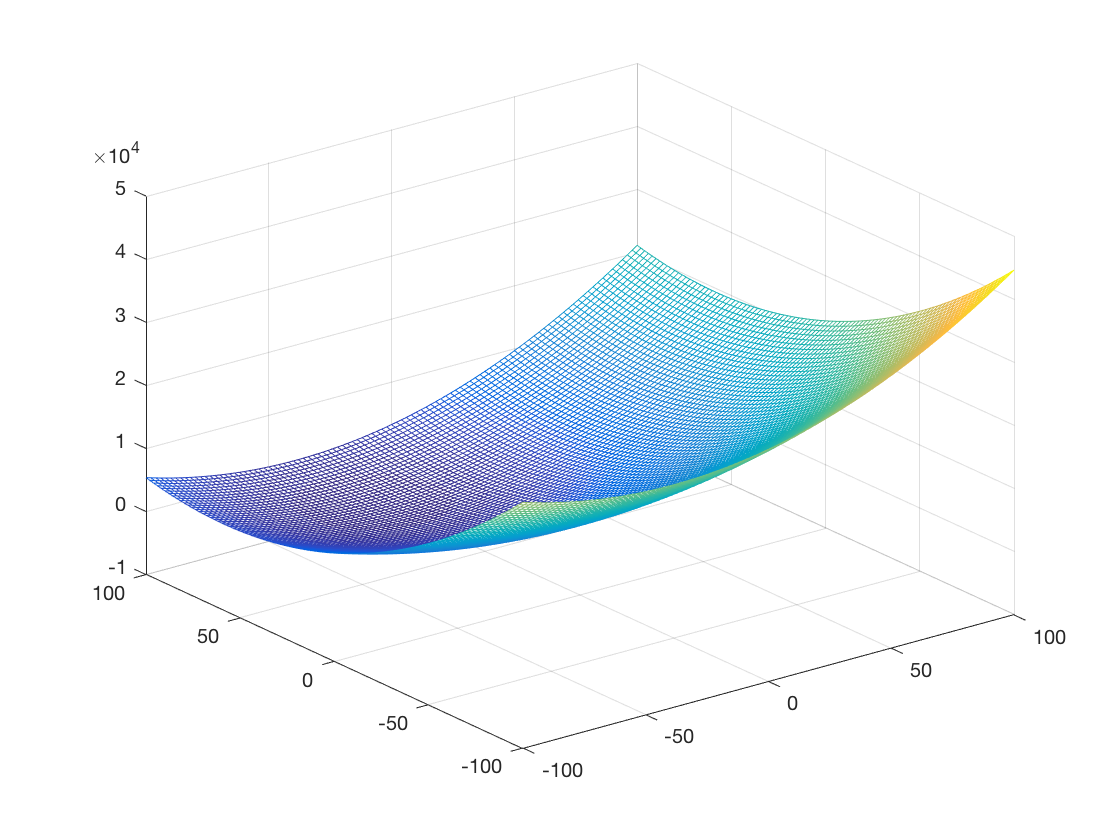
\includegraphics[width=.5\linewidth]{f1}
  \caption{3-D map for 2-D function}
  \label{f1}
\end{figure}

\subsubsection{$F_2$: Shifted Schwefel’s Problem}

\begin{equation}
  F_2(x)=\sum_{i=1}^{D}{(\sum_{j=1}^{i}{z_j})^2}
\end{equation}
\[ z=x-o \]
\[ x \in [-100,100]^D \]

\begin{figure}[H]
  \centering
  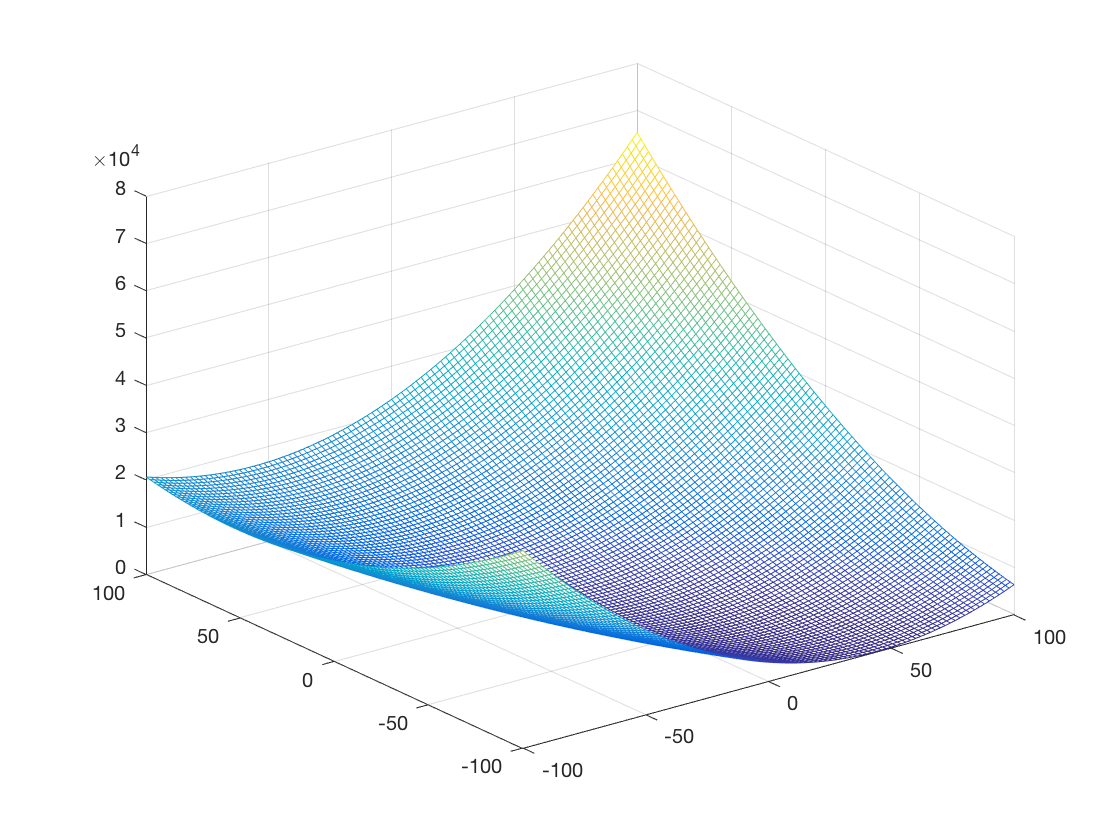
\includegraphics[width=.5\linewidth]{f2}
  \caption{3-D map for 2-D function}
  \label{f2}
\end{figure}

\subsubsection{$F_3$: Shifted Rotated High Conditioned Elliptic Function}

\begin{equation}
  F_3(x)=\sum_{i=1}^{D}{(10^6)^{\frac{i-1}{D-1}}z_i^2}
\end{equation}
\[ z=(x-o)*M \]
\[ x \in [-100,100]^D \]

\begin{figure}[H]
  \centering
  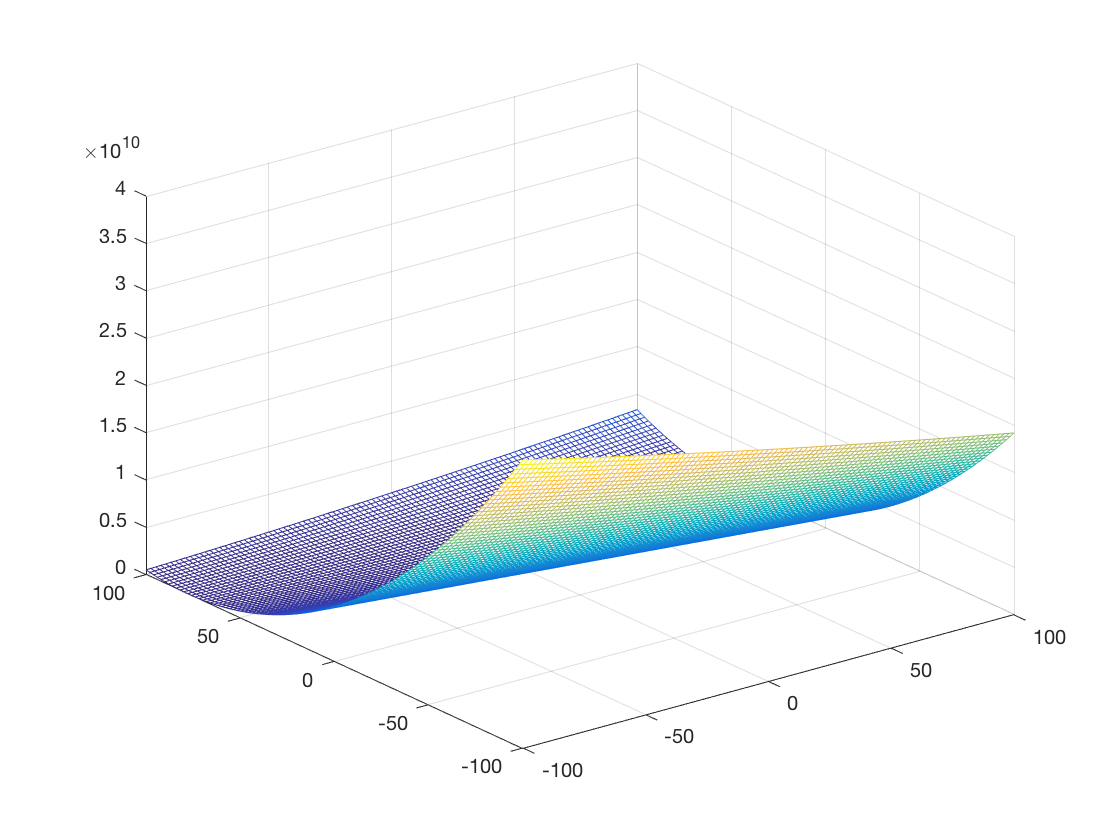
\includegraphics[width=.5\linewidth]{f3}
  \caption{3-D map for 2-D function}
  \label{f3}
\end{figure}

\subsubsection{$F_4$: Shifted Schwefel’s Problem with Noise in Fitness}

\begin{equation}
  F_4(x)=(\sum_{i=1}^{D}{(\sum_{j=1}^{i}{z_j})^2})*(1+0.4|N(0,1)|)
\end{equation}
\[ z=x-o \]
\[ x \in [-100,100]^D \]

\begin{figure}[H]
  \centering
  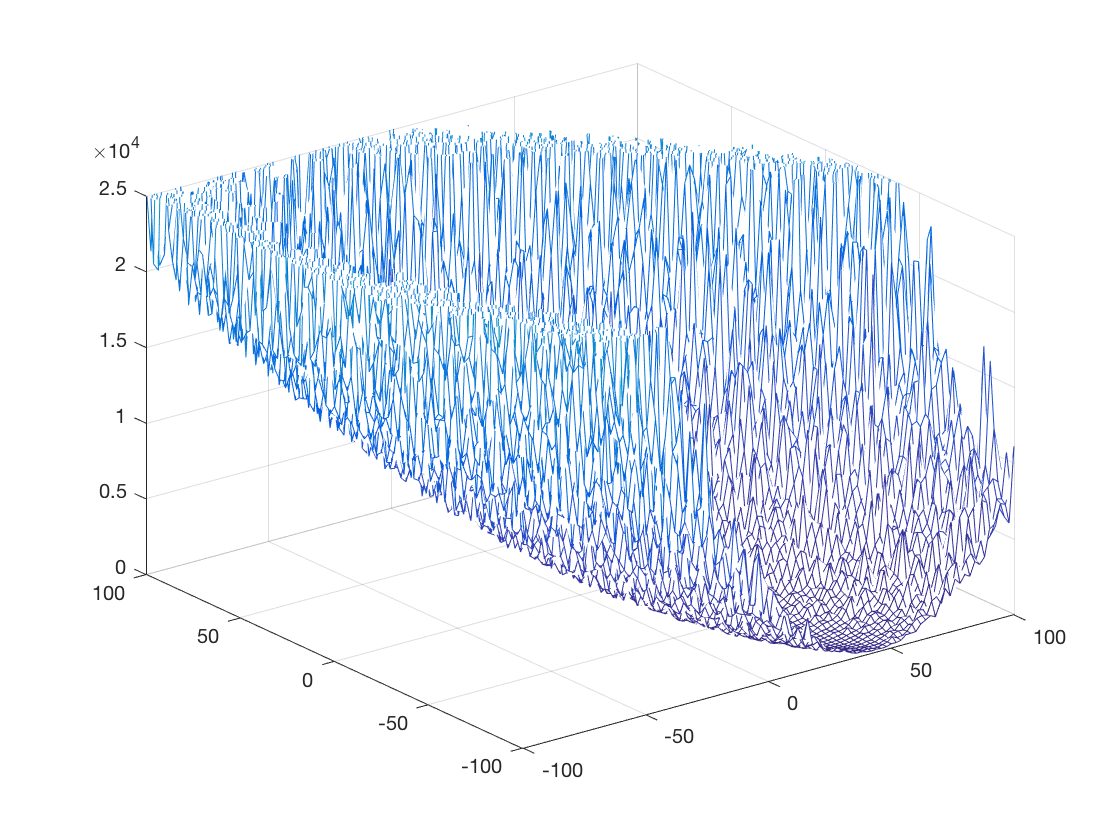
\includegraphics[width=.5\linewidth]{f4}
  \caption{3-D map for 2-D function}
  \label{f4}
\end{figure}

\subsubsection{$F_5$: Schwefel’s Problem with Global Optimum on Bounds}

\begin{equation}
  F_5(x)=max\{|A_ix-B_i|\}
\end{equation}
\[ i=1,...,D, x \in [-100,100]^D \]
\[ A \text{ is a } D*D \text{ matrix}, a_{ij} = \text{ random numbers in } [-500,500],  det(A) \neq 0 \]
\[ B_i = A_i * o, o_i = \text{ random numbers in } [-100,100] \]
\[ o_i = -100 \text{, for } i=1,2,...,[D/4], o_i = 100 \text{, for } i=[3D/4],...,D \]

\begin{figure}[H]
  \centering
  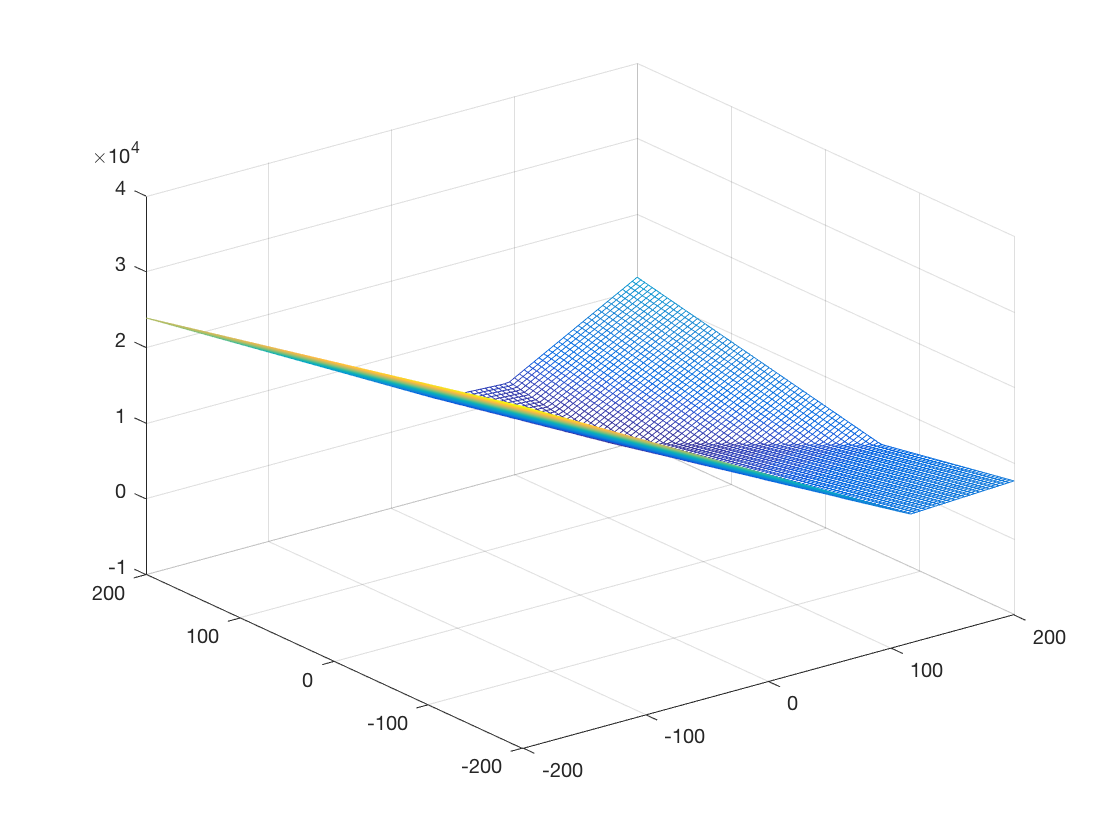
\includegraphics[width=.5\linewidth]{f5}
  \caption{3-D map for 2-D function}
  \label{f5}
\end{figure}

\subsubsection{$F_6$: Shifted Rosenbrock’s Function}

\begin{equation}
  F_6(x)=\sum_{i=1}^{D-1}{(100(z_i^2 - z_{i+1})^2 + (z_i - 1)^2)}
\end{equation}
\[ z=x-o+1 \]
\[ x \in [-100,100]^D \]

\begin{figure}[H]
  \centering
  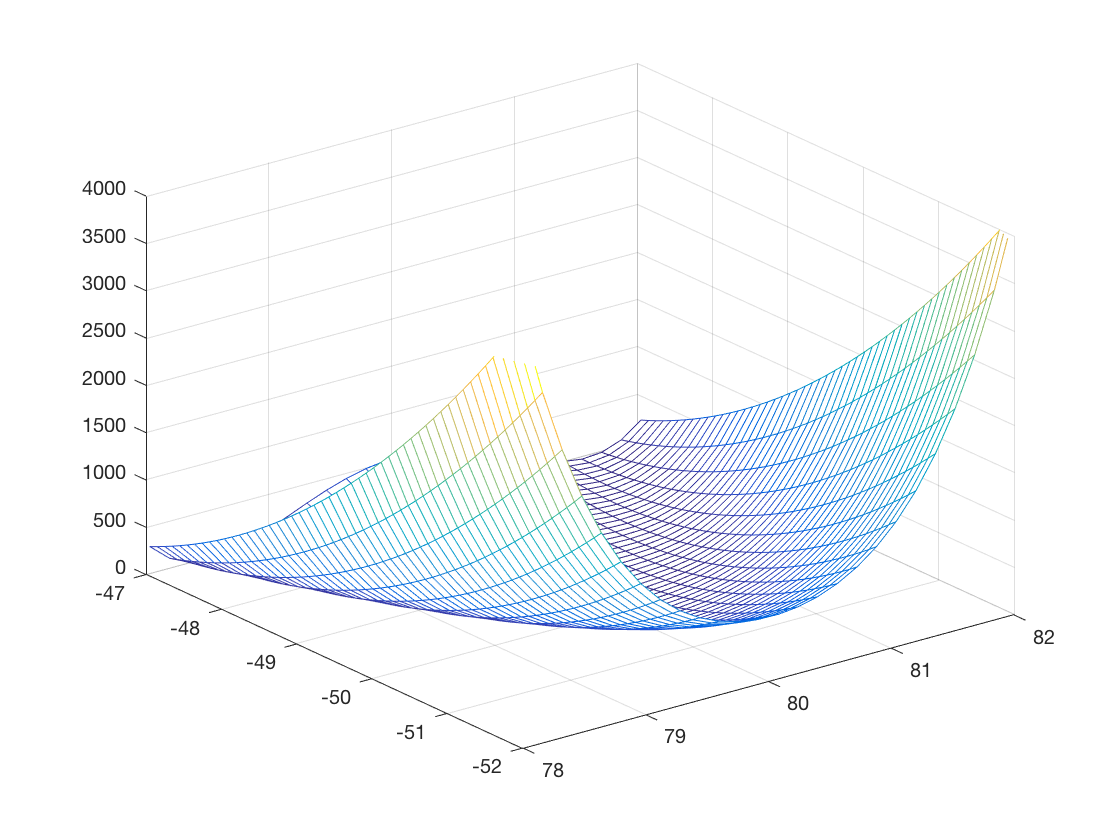
\includegraphics[width=.5\linewidth]{f6}
  \caption{3-D map for 2-D function}
  \label{f6}
\end{figure}

\subsubsection{$F_7$: Shifted Rotated Griewank’s Function without Bounds}

\begin{equation}
  F_7(x)=\sum_{i=1}^{D}{\frac{z_i^2}{4000}}-\prod_{i=1}^{D}{\cos{\frac{z_i}{\sqrt{i}}}}+1
\end{equation}
\[ z=(x-o)*M \]
\[ x \in [0,600]^D \]

\begin{figure}[H]
  \centering
  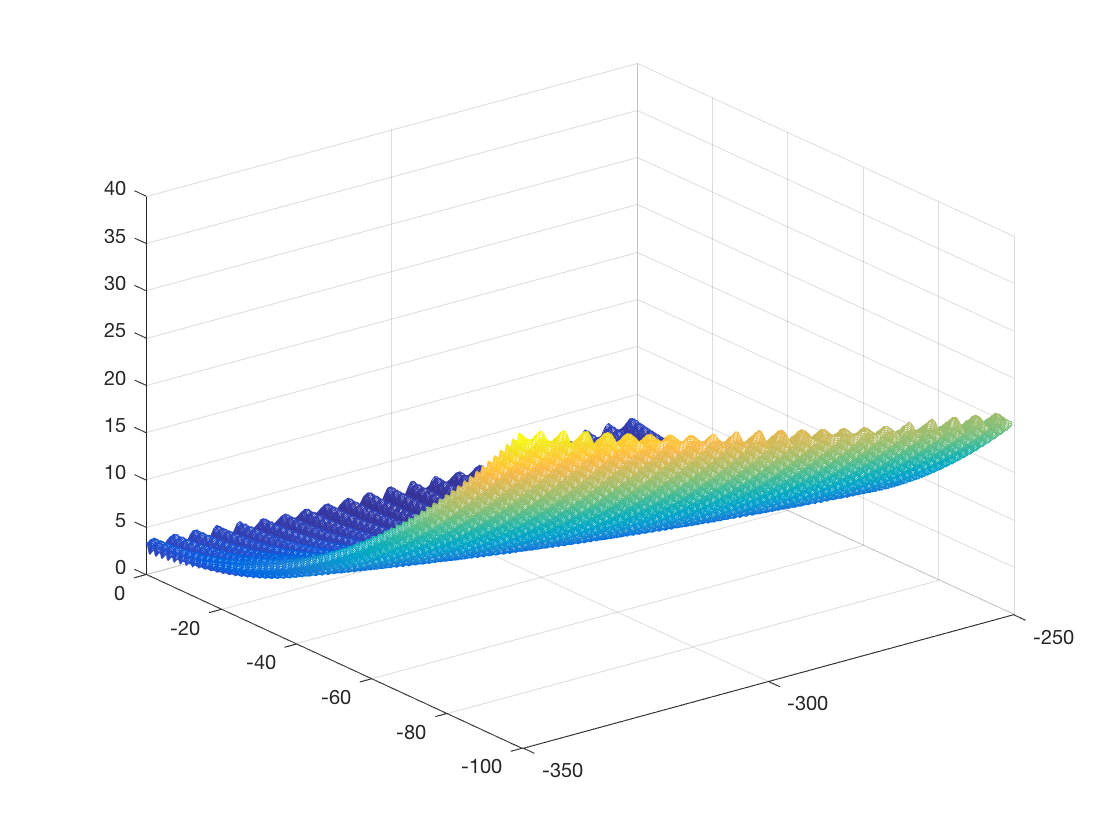
\includegraphics[width=.5\linewidth]{f7}
  \caption{3-D map for 2-D function}
  \label{f7}
\end{figure}

\subsubsection{$F_8$: Shifted Rotated Ackley’s Function with Global Optimum on Bounds}

\begin{equation}
  F_8(x)=-20\exp{(-0.2\sqrt{\frac{1}{D}\sum_{i=1}^{D}{z_i^2}})}-\exp{(\frac{1}{D}\sum_{i=1}^{D}{\cos{(2\pi z_i)}})} + 20 + e
\end{equation}
\[ z=(x-o)*M \]
\[ x \in [-32,32]^D \]

\begin{figure}[H]
  \centering
  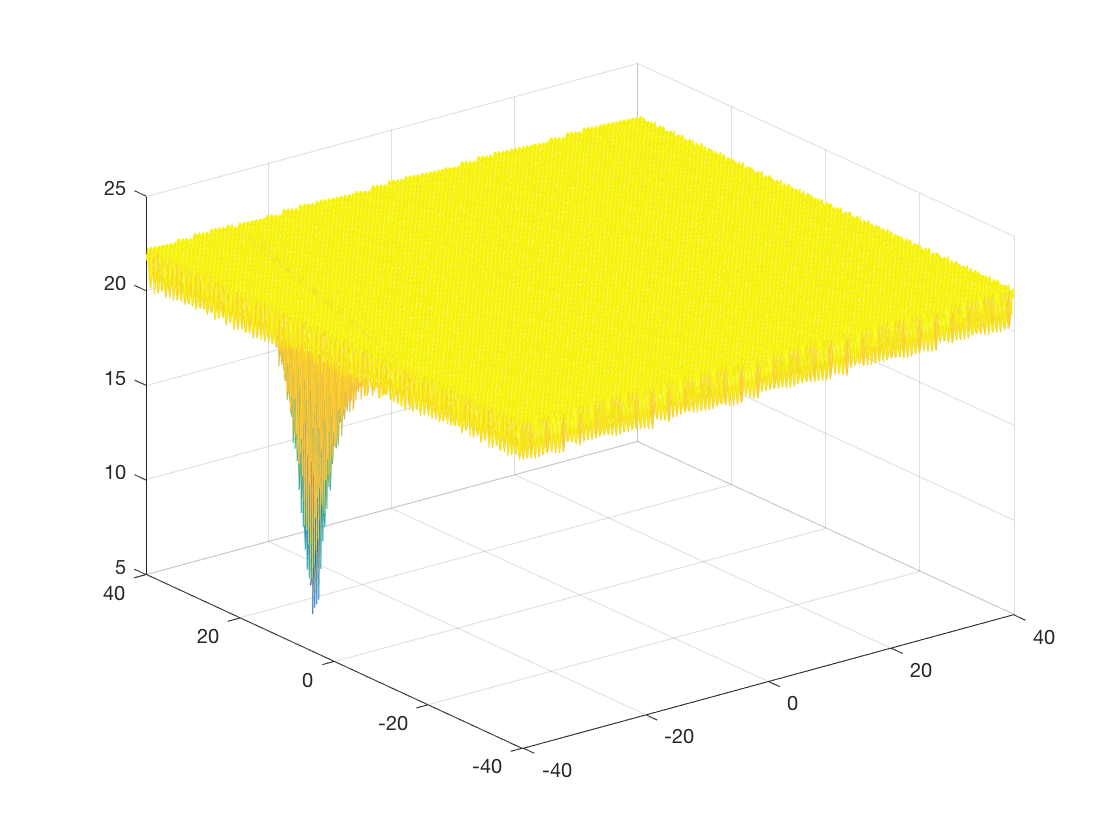
\includegraphics[width=.5\linewidth]{f8}
  \caption{3-D map for 2-D function}
  \label{f8}
\end{figure}

\subsubsection{$F_9$: Shifted Rastrigin’s Function}

\begin{equation}
  F_9(x)=\sum_{i=1}^{D}{z_i^2 - 10\cos{(2\pi z_i)} + 10}
\end{equation}
\[ z=x-o \]
\[ x \in [-5,5]^D \]

\begin{figure}[H]
  \centering
  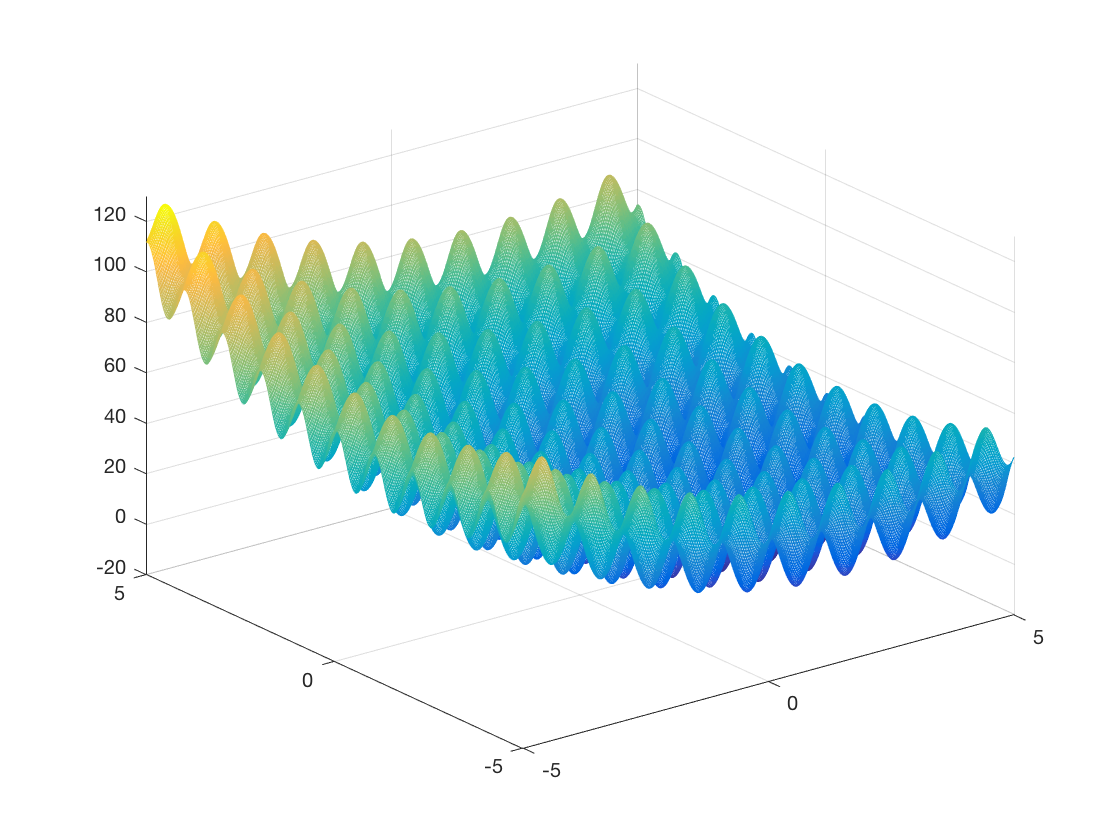
\includegraphics[width=.5\linewidth]{f9}
  \caption{3-D map for 2-D function}
  \label{f9}
\end{figure}

\subsubsection{$F_{10}$: Shifted Rotated Rastrigin’s Function}

\begin{equation}
  F_{10}(x)=\sum_{i=1}^{D}{z_i^2 - 10\cos{(2\pi z_i)} + 10}
\end{equation}
\[ z=(x-o)*M \]
\[ x \in [-5,5]^D \]

\begin{figure}[H]
  \centering
  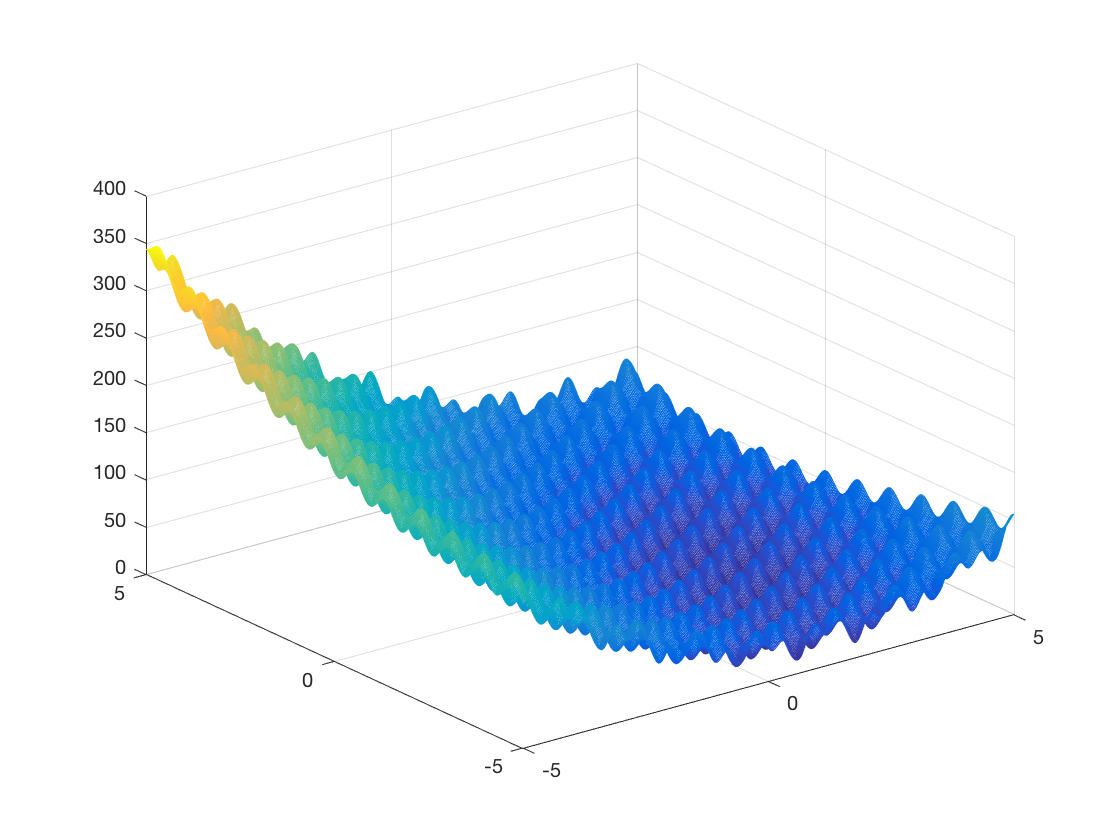
\includegraphics[width=.5\linewidth]{f10}
  \caption{3-D map for 2-D function}
  \label{f10}
\end{figure}

\subsection{Training neural networks}

Artificial neural networks usually consist of the following components:

\begin{enumerate}
  \item A graf of nodes (neurons) and links between nodes
  \item A variable for each neuron which contains it's value
  \item A real weight for each link between nodes
  \item A real threshold for each node
  \item A transfer function which calculates the value of each neuron based on other neurons variables, link-weights and thresholds
\end{enumerate}

Feed-Forward neural networks contain one level of input-nodes, one or more levels of hidden nodes and one level of output-nodes. The input-nodes accept an incomming singla vector and the output-neurons transmit the output-vector back to the user. All node in each level are linked to all other nodes in the previous and next levels \cite{montana1989training}. See figure \ref{figure:FFNN} for an illustration of a simple FFNN with two input nodes ($z_1$ and $z_2$), three hidden nodes ($y_1$, $y_2$ och $y_3$), two ouput nodes ($o_1$ och $o_2$) and weights between them represented by $v_{ij}$ and $w_{ij}$.

\subsubsection{Evaluating the network}

The value of neuron $x_i$ in the network is calculated according to the following equations

\begin{equation}
  x_i = f(\xi_i)
  \label{neuron}
\end{equation}

\begin{equation}
  \xi_i = v_i + \sum_{j = 0}^{n} {\omega_{ij}x_{j}}
  \label{neuron_sum}
\end{equation}

\noindent
where $n$ is the number of neurons in the previous layer, $x_j$ are neurons in the previous layer and $v_i$ are the weights between $x_i$ and $x_j$.

The function $f$ is the transfer-function and is defined according to

\begin{equation}
  f(\xi) = \frac {1} {1 + exp(-\xi)}
\end{equation}

To simplify the notation the threshold is added to the network as an additional node to all layers except the output-layer with a constant value of $-1$. The threshold values are the determined by the outgoing weights from the threshold nodes \cite{svozil1997introduction}.



\begin{figure}[H]
  \centering
    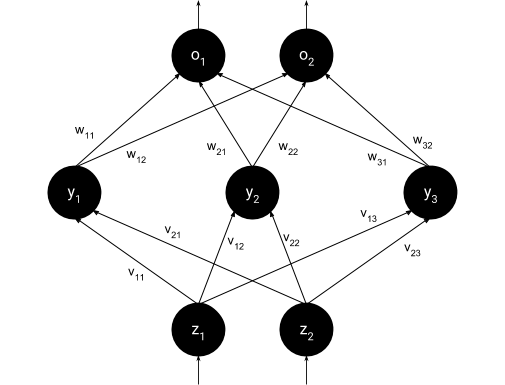
\includegraphics[width=10cm]{FFNN}
  \caption{Feed-Forward Neural Network}
  \label{figure:FFNN}
\end{figure}


\subsubsection{Backpropagation}

Backpropagation is the most popular method to train neural networks. Training-data is sent through the network and the result-vector is subtracted from the correct output-vector, squared and summed. The sum of squared differences is the propagated back through the network assigning a delta value to each node. Then new weights are calculated for each link based on the nodes delta values and the derivative of the transfer function. After a large enough number iterations the network will have learnt to correctly process the traning data and make correct predictions for all data in general \cite{engelbrecht2007computational}.

%\newpage


% ============================= Final words ============================
\newpage
\section{Results}

This section presents benchmarks and measurements of the four main algorithms presented in this thesis. It is divided into two parts: the function optimization benchmark and the machine learning benchmark.

\subsection{Mathematical Problem Set}

The function test-bed was tested with dimension size $D=10$, $D=30$ and $D=50$. The parameters for different dimension sizes are presented in figure~\ref{t1}.

\begin{figure}[H]
  \centering
  \begin{center}
    \begin{tabular}{ | l | c | r | }
      \hline
      Dimension & Max. Generations & Population size \\ \hline
      10 & 667 & 150 \\ \hline
      30 & 1200 & 250 \\ \hline
      50 & 1429 & 350 \\
      \hline
    \end{tabular}
  \end{center}
  \caption{Parameters for different dimension sizes in the benchmark}
  \label{t1}
\end{figure}

The benchmark ran each test-case 30 times and recorded the average minimum value of the function and the standard deviation. The results are presented in figure~\ref{r10},~\ref{r30} and~\ref{r50}. The lowest value is marked in bold font.




\begin{figure}[H]
  \centering
  \begin{center}
    \footnotesize
    \begin{tabular}{ | c | c | c | c | c | c | c | c | c | }
      \hline
      F & \multicolumn{2}{c|}{DE} & \multicolumn{2}{c|}{PSO} & \multicolumn{2}{c|}{EDA} & \multicolumn{2}{c |}{DEDA} \\ \hline
      & Avg & Std & Avg & Std & Avg & Std & Avg & Std \\ \hline
      1 & 3,88E-17 & 3,42E-17 & 1,65E-16 & 3,64E-16 & \textbf{1,67E-27} & 4,07E-28 & 0,00E+00 & 0,00E+00 \\ \hline
      2 & 1,83E-08 & 1,24E-08 & 2,07E-06 & 3,36E-06 & 2,51E+02 & 1,42E+02 & \textbf{4,23E-27} & 3,10E-27 \\ \hline
      3 & 5,19E-01 & 2,29E-01 & 4,88E+05 & 7,21E+05 & 1,09E+05 & 8,32E+04 & \textbf{4,96E-02} & 3,01E-02 \\ \hline
      4 & 3,36E-07 & 2,59E-07 & 6,31E-05 & 9,10E-05 & 3,21E+02 & 2,16E+02 & \textbf{1,73E-26} & 2,16E-26 \\ \hline
      5 & \textbf{4,24E-13} & 7,82E-13 & 4,94E+02 & 4,49E+02 & 1,67E+02 & 1,37E+02 & 6,57E+00 & 1,26E+01 \\ \hline
      6 & \textbf{5,43E-05} & 1,24E-04 & 2,11E+02 & 7,15E+02 & 1,34E+04 & 4,30E+04 & 6,71E+00 & 5,83E-01 \\ \hline
      7 & 4,87E-01 & 7,61E-02 & 2,74E-01 & 1,79E-01 & \textbf{1,87E-01} & 2,23E-01 & 3,41E-01 & 1,24E-01 \\ \hline
      8 & 2,04E+01 & 7,20E-02 & \textbf{2,03E+01} & 8,82E-02 & 2,04E+01 & 8,15E-02 & 2,04E+01 & 6,88E-02 \\ \hline
      9 & 2,50E+01 & 4,44E+00 & \textbf{1,76E+00} & 1,49E+00 & 2,35E+01 & 3,08E+00 & 1,80E+01 & 3,52E+00 \\ \hline
      10 & 3,26E+01 & 4,25E+00 & \textbf{1,73E+01} & 7,50E+00 & 2,11E+01 & 3,43E+00 & 2,05E+01 & 3,62E+00 \\ \hline
    \end{tabular}
  \end{center}
  \caption{Benchmark results for $D=10$}
  \label{r10}
\end{figure}

\begin{figure}[H]
  \centering
  \begin{center}
    \footnotesize
    \begin{tabular}{ | c | c | c | c | c | c | c | c | c | }
      \hline
      F & \multicolumn{2}{c|}{DE} & \multicolumn{2}{c|}{PSO} & \multicolumn{2}{c|}{EDA} & \multicolumn{2}{c |}{DEDA} \\ \hline
      & Avg & Std & Avg & Std & Avg & Std & Avg & Std \\ \hline
      1 & 1,03E+00 & 1,53E-01 & 4,54E-10 & 7,66E-10 & 1,81E-25 & 7,66E-10 & \textbf{8,58E-28} & 1,40E-28 \\ \hline
      2 & 3,07E+03 & 6,91E+02 & 1,42E+03 & 7,01E+02 & 1,71E+03 & 7,01E+02 & \textbf{4,84E+02} & 1,80E+02 \\ \hline
      3 & 3,28E+07 & 5,84E+06 & 1,92E+07 & 1,12E+07 & 4,93E+06 & 1,12E+07 & 1,88E+07 & 4,86E+06 \\ \hline
      4 & 6,06E+03 & 1,23E+03 & 1,50E+04 & 6,87E+03 & \textbf{3,63E+03} & 6,87E+03 & \textbf{6,74E+02} & 1,96E+02 \\ \hline
      5 & 1,38E+03 & 3,54E+02 & 6,92E+03 & 2,55E+03 & 2,70E+03 & 2,55E+03 & \textbf{1,31E+02} & 9,21E+01 \\ \hline
      6 & 2,99E+03 & 1,24E+03 & \textbf{5,30E+02} & 8,60E+02 & 8,57E+04 & 8,60E+02 & 7,32E+03 & 2,21E+04 \\ \hline
      7 & 1,22E+00 & 5,36E-02 & \textbf{5,77E-02} & 5,18E-02 & 5,86E+00 & 5,18E-02 & 2,54E-01 & 4,25E-01 \\ \hline
      8 & 2,09E+01 & 4,24E-02 & \textbf{2,09E+01} & 5,74E-02 & 2,10E+01 & 5,74E-02 & 2,10E+01 & 5,41E-02 \\ \hline
      9 & 1,91E+02 & 9,58E+00 & \textbf{2,53E+01} & 5,97E+00 & 1,53E+02 & 5,97E+00 & 1,60E+02 & 8,27E+00 \\ \hline
      10 & 2,19E+02 & 1,09E+01 & \textbf{1,14E+02} & 3,78E+01 & 1,59E+02 & 3,78E+01 & 1,60E+02 & 8,53E+00 \\ \hline
    \end{tabular}
  \end{center}
  \caption{Benchmark results for $D=30$}
  \label{r30}
\end{figure}

\begin{figure}[H]
  \centering
  \begin{center}
    \footnotesize
    \begin{tabular}{ | c | c | c | c | c | c | c | c | c | }
      \hline
      F & \multicolumn{2}{c|}{DE} & \multicolumn{2}{c|}{PSO} & \multicolumn{2}{c|}{EDA} & \multicolumn{2}{c |}{DEDA} \\ \hline
      & Avg & Std & Avg & Std & Avg & Std & Avg & Std \\ \hline
      1 & 5,64E+02 & 8,54E+01 & 1,20E-04 & 1,49E-04 & 1,04E-24 & 9,53E-26 & \textbf{2,14E-26} & 4,42E-27 \\ \hline
      2 & 5,00E+04 & 4,88E+03 & 3,69E+04 & 1,02E+04 & \textbf{3,55E+03} & 6,45E+02 & 3,96E+04 & 5,00E+03 \\ \hline
      3 & 2,52E+08 & 3,33E+07 & 8,68E+07 & 4,64E+07 & \textbf{1,31E+07} & 2,94E+06 & 1,96E+08 & 3,16E+07 \\ \hline
      4 & 7,02E+04 & 9,89E+03 & 1,12E+05 & 3,09E+04 & \textbf{8,17E+03} & 1,71E+03 & 5,08E+04 & 7,70E+03 \\ \hline
      5 & 1,33E+04 & 1,03E+03 & 1,48E+04 & 3,64E+03 & 4,31E+03 & 2,95E+02 & \textbf{2,71E+03} & 3,84E+02 \\ \hline
      6 & 7,19E+06 & 2,18E+06 & 1,62E+04 & 3,11E+04 & \textbf{1,18E+04} & 2,68E+04 & 2,23E+04 & 1,09E+05 \\ \hline
      7 & 3,32E+01 & 6,43E+00 & 1,05E+00 & 1,24E-01 & 1,25E+01 & 3,91E+00 & \textbf{6,04E-01} & 6,19E-01 \\ \hline
      8 & 2,12E+01 & 2,28E-02 & \textbf{2,11E+01} & 5,09E-02 & 2,11E+01 & 4,97E-02 & 2,11E+01 & 3,28E-02 \\ \hline
      9 & 3,94E+02 & 1,24E+01 & \textbf{7,93E+01} & 1,46E+01 & 3,14E+02 & 1,41E+01 & 3,27E+02 & 1,13E+01 \\ \hline
      10 & 4,48E+02 & 1,87E+01 & \textbf{2,79E+02} & 6,36E+01 & 3,20E+02 & 1,17E+01 & 3,27E+02 & 9,26E+00 \\ \hline
    \end{tabular}
  \end{center}
  \caption{Benchmark results for $D=50$}
  \label{r50}
\end{figure}


\subsection{Machine Learning Problem Set}

\subsubsection{$ML_{4}$: Neuroevolution of Game Controller for ``Snake''}

The $ML_{4}$ results are shown in figure \ref{ml4}. The parameters are shown in figure \ref{ml4_p}.

\begin{figure}[H]
  \centering
  \begin{center}
    \footnotesize
    \begin{tabular}{ | l | l| }
      \hline
      Parameter & Value \\ \hline
      Individuals & 140 \\ \hline
      Generations & 1000 \\ \hline
      Grid dimension & 10*10 \\ \hline
      Weight dimension & 140 \\ \hline
      Repeat measurements & 10 \\ \hline
      Repeat fitness measurements & 5 \\ \hline
    \end{tabular}
  \end{center}
  \caption{Benchmark parameters for $ML_{4}$}
  \label{ml4_p}
\end{figure}

\begin{figure}[H]
  \centering
  \begin{center}
    \footnotesize
    \begin{tabular}{ | c | c | c | c | c | c | c | c | c | }
      \hline
      F & \multicolumn{2}{c|}{DE} & \multicolumn{2}{c|}{PSO} & \multicolumn{2}{c|}{EDA} & \multicolumn{2}{c |}{DEDA} \\ \hline
       & Avg & Std & Avg & Std & Avg & Std & Avg & Std \\ \hline
      snake & 2,32E+01 & 2,19E+00 & 2,92E+01 & 4,16E+00 & 2,78E+01 & 1,34E+01 & 2,69E+01 & 3,59E+00 \\ \hline
    \end{tabular}
  \end{center}
  \caption{Benchmark results for $ML_{4}$}
  \label{ml4}
\end{figure}

\subsubsection{$ML_{1-3}$: Sample Data Sets}


The algorithms were tested on four machine learning benchmarks: $ML_{1}$, $ML_{2}$, $ML_{3}$ and $ML_{4}$ as described in the section ``Method''. The dimensionality of the problem depends on the size of the input and output vectors of the data-sets and the size of the hidden layer of the neural networks. The hidden layer size was defines as the mean of the input- and output-layer sizes. The population size was set to $50$, the max. number of generations was set to $100$ and every measurement was made $5$ times. The figures~\ref{ml1},~\ref{ml2},~\ref{ml3} and~\ref{ml4} show the results obtained for problems (average minimum value and standard deviation).


\begin{figure}[H]
  \centering
  \begin{center}
    \footnotesize
    \begin{tabular}{ | c | c | c | c | c | c | c | c | c | }
      \hline
      F & \multicolumn{2}{c|}{DE} & \multicolumn{2}{c|}{PSO} & \multicolumn{2}{c|}{EDA} & \multicolumn{2}{c |}{DEDA} \\ \hline
       & Avg & Std & Avg & Std & Avg & Std & Avg & Std \\ \hline
      simplefit\_dataset & 0 & 0 & 0 & 0 & 0 & 0 & 0 & 0 \\ \hline
      abalone\_dataset & 0 & 0 & 0 & 0 & 0 & 0 & 0 & 0 \\ \hline
      bodyfat\_dataset & 0 & 0 & 0 & 0 & 0 & 0 & 0 & 0 \\ \hline
      building\_dataset & 0 & 0 & 0 & 0 & 0 & 0 & 0 & 0 \\ \hline
      chemical\_dataset & 0 & 0 & 0 & 0 & 0 & 0 & 0 & 0 \\ \hline
      cho\_dataset & 0 & 0 & 0 & 0 & 0 & 0 & 0 & 0 \\ \hline
      engine\_dataset & 0 & 0 & 0 & 0 & 0 & 0 & 0 & 0 \\ \hline
      house\_dataset & 0 & 0 & 0 & 0 & 0 & 0 & 0 & 0 \\ \hline
    \end{tabular}
  \end{center}
  \caption{Benchmark results for $ML_{1}$}
  \label{ml1}
\end{figure}

\begin{figure}[H]
  \centering
  \begin{center}
    \footnotesize
    \begin{tabular}{ | c | c | c | c | c | c | c | c | c | }
      \hline
      F & \multicolumn{2}{c|}{DE} & \multicolumn{2}{c|}{PSO} & \multicolumn{2}{c|}{EDA} & \multicolumn{2}{c |}{DEDA} \\ \hline
       & Avg & Std & Avg & Std & Avg & Std & Avg & Std \\ \hline
      simpleclass\_dataset & 0 & 0 & 0 & 0 & 0 & 0 & 0 & 0 \\ \hline
      cancer\_dataset & 0 & 0 & 0 & 0 & 0 & 0 & 0 & 0 \\ \hline
      crab\_dataset & 0 & 0 & 0 & 0 & 0 & 0 & 0 & 0 \\ \hline
      glass\_dataset & 0 & 0 & 0 & 0 & 0 & 0 & 0 & 0 \\ \hline
      iris\_dataset & 0 & 0 & 0 & 0 & 0 & 0 & 0 & 0 \\ \hline
      thyroid\_dataset & 0 & 0 & 0 & 0 & 0 & 0 & 0 & 0 \\ \hline
      wine\_dataset & 0 & 0 & 0 & 0 & 0 & 0 & 0 & 0 \\ \hline
    \end{tabular}
  \end{center}
  \caption{Benchmark results for $ML_{2}$}
  \label{ml2}
\end{figure}

\begin{figure}[H]
  \centering
  \begin{center}
    \footnotesize
    \begin{tabular}{ | c | c | c | c | c | c | c | c | c | }
      \hline
      F & \multicolumn{2}{c|}{DE} & \multicolumn{2}{c|}{PSO} & \multicolumn{2}{c|}{EDA} & \multicolumn{2}{c |}{DEDA} \\ \hline
       & Avg & Std & Avg & Std & Avg & Std & Avg & Std \\ \hline
      simplecluster\_dataset & 0 & 0 & 0 & 0 & 0 & 0 & 0 & 0 \\ \hline
    \end{tabular}
  \end{center}
  \caption{Benchmark results for $ML_{3}$}
  \label{ml3}
\end{figure}

\newpage
\section{Discussions}

Lorem ipsum dolor sit amet, consectetur adipiscing elit. Sed suscipit eu ante id aliquet. Class aptent taciti sociosqu ad litora torquent per conubia nostra, per inceptos himenaeos. Mauris condimentum iaculis erat, eget pretium leo consequat eget. Donec eu aliquam purus. Quisque scelerisque feugiat ligula, non vehicula urna blandit nec. Etiam a dignissim purus, at molestie dui. Vestibulum a venenatis mi, id hendrerit sem. Cras purus elit, dapibus eget est id, lacinia tincidunt neque. Mauris eu arcu ipsum. Sed enim leo, iaculis vitae nisl tincidunt, ultricies accumsan diam. Donec neque urna, pellentesque sit amet interdum a, pretium ac enim. Proin quis ante nunc. Fusce vitae lorem condimentum, porta velit blandit, commodo nisi.

\newpage
\section{Conclusions}

{\color{blue} I detta avsnitt ska du summera rapporten samt presentera slutsatser och slutanalys. Ge en kort \"oversikt av syftet och fr\r{a}gest\"allningen. Du ska sedan tydligt tala om de viktigaste resultaten, f\"orklara deras signifikans och s\"atta in dem i sitt sammanhang. Alla slutsatser ska ha st\"od i tidigare delar av rapporten.  Du ska d\"aremot inte presentera nya detaljer.

En expert ska kunna l\"asa detta avsnitt oberoende av resten av rapporten. }

\newpage
\section{Acknowledgments}

Lorem ipsum dolor sit amet, consectetur adipiscing elit. Sed suscipit eu ante id aliquet. Class aptent taciti sociosqu ad litora torquent per conubia nostra, per inceptos himenaeos. Mauris condimentum iaculis erat, eget pretium leo consequat eget. Donec eu aliquam purus. Quisque scelerisque feugiat ligula, non vehicula urna blandit nec. Etiam a dignissim purus, at molestie dui. Vestibulum a venenatis mi, id hendrerit sem. Cras purus elit, dapibus eget est id, lacinia tincidunt neque. Mauris eu arcu ipsum. Sed enim leo, iaculis vitae nisl tincidunt, ultricies accumsan diam. Donec neque urna, pellentesque sit amet interdum a, pretium ac enim. Proin quis ante nunc. Fusce vitae lorem condimentum, porta velit blandit, commodo nisi.


%\input{./outcome}

%\input{./timeplan}
% ============================= References ============================
\newpage
\bibliographystyle{IEEEtran}
\bibliography{./references}
\addcontentsline{toc}{section}{References}

% ============================ Appendices =============================
%\newpage
%\begin{appendices}

	%\section{Algorithms}

This appendix will present the matlab code for the four algorithms descibed under ``Algorithms''.

\subsection{Differential Evolution}

\inputminted{C}{DE.m}

	%\clearpage

	%\input{./Appendices/appendices2}
	%\clearpage

%\end{appendices}

\end{document}
